\documentclass[11pt]{article}

\usepackage[margin=1in]{geometry}
\usepackage[T1]{fontenc}
\usepackage[utf8]{inputenc}
\usepackage{lmodern}
\usepackage{microtype}
\usepackage{amsmath,amssymb,amsthm,mathtools}
\usepackage{booktabs}
\usepackage{longtable}
\usepackage{tabularx}
\usepackage{array}
\usepackage{enumitem}
\usepackage{fancyvrb}
\usepackage{fvextra}
\usepackage{xcolor}
\usepackage{hyperref}
\usepackage{xurl}
\usepackage{tikz}
\usetikzlibrary{arrows.meta,positioning,fit,calc,shapes.geometric,shapes.multipart}

\hypersetup{
  colorlinks=true,
  linkcolor=blue!50!black,
  urlcolor=blue!50!black,
  citecolor=blue!50!black,
  pdftitle={Asymptote Fault Tolerance (AFT): Universally Breaking the Lower Bound with Relay-Free Deterministic 99\% Byzantine Fault Tolerance},
  pdfauthor={IOI}
}

\newtheorem{theorem}{Theorem}
\newtheorem{proposition}{Proposition}

\newcommand{\AFT}{\textsc{AFT}}
\newcommand{\code}[1]{\texttt{#1}}
\newcommand{\term}[1]{\textit{#1}}
\newcommand{\suchthat}{\;|\;}
\definecolor{artifactframe}{RGB}{52,73,94}
\definecolor{artifactfill}{RGB}{246,249,252}
\definecolor{artifacttitlefill}{RGB}{232,239,245}
\newcommand{\doctrinebox}[1]{%
\medskip
\noindent\begingroup
\setlength{\fboxsep}{8pt}%
\fcolorbox{artifactframe}{artifactfill}{\parbox{\dimexpr\linewidth-2\fboxsep-2\fboxrule}{#1}}%
\endgroup
\medskip
}
\newcommand{\artifactgroup}[2]{%
\clearpage
\subsection{#1}
\noindent\begingroup
\setlength{\fboxsep}{8pt}%
\colorbox{artifacttitlefill}{\parbox{\dimexpr\linewidth-2\fboxsep}{#2}}%
\endgroup
\par\medskip
}
\newcommand{\embedartifact}[4]{%
\subsubsection{\code{#1}}
\label{#2}
\noindent\begingroup
\setlength{\fboxsep}{6pt}%
\colorbox{artifactfill}{\parbox{\dimexpr\linewidth-2\fboxsep}{\textbf{Repository path.} \path{#3}}}%
\endgroup

\medskip
\VerbatimInput[
  fontsize=\footnotesize,
  baselinestretch=0.94,
  breaklines=true,
  breakanywhere=true,
  numbers=left,
  numbersep=8pt,
  frame=single,
  framerule=0.3pt,
  rulecolor=\color{artifactframe},
  framesep=5pt
]{#4}
}

\setlength{\emergencystretch}{3em}

\title{Asymptote Fault Tolerance (AFT): Universally Breaking the Lower Bound with Relay-Free Deterministic 99\% Byzantine Fault Tolerance}
\author{IOI}
\date{March 17, 2026}

\begin{document}

\maketitle

\begin{abstract}
Asymptote Fault Tolerance (\AFT{}) is a family of consensus and settlement constructions for
high-throughput ordering, guardian-backed base finality, proof-carrying
canonical ordering, and deterministic release of irreversible effects. Its
central move is to stop treating dense positive voting as the only possible
source of ordering truth. Instead, \AFT{} separates throughput-critical
publication and chain progression from authority-critical proof verification,
omission detection, and effect collapse.

The protocol family has four interacting surfaces. \term{GuardianMajority}
supplies the production base-finality path: a validator quorum certificate is
necessary but not sufficient, because each proposal must also carry a
registered guardian committee certificate anchored into shared evidence.
\term{CanonicalOrdering} supplies the proof-carrying ordering path: a slot
order is accepted because a canonical certificate is uniquely valid and
recoverable from public inputs, not because a dense validator quorum voted the
order into existence. \term{Asymptote} supplies the sealing path for
irreversible effects: \code{BaseFinal} chain progress is upgraded to
\code{SealedFinal} through deterministic witness or observer-backed collapse,
with canonical observer challenges dominating unsafe releases.
\term{NestedGuardian} supplies a
witness-augmented mode for layered threshold constructions.

This paper is self-contained and normative for the protocol family. Its
ordering subtheorem remains \code{99\%} equal-authority ordering consensus
under explicit bulletin-publication, cutoff, omission, protocol-native
retrievability, and proof-soundness assumptions. The runtime also
internalizes compact signed publication-frontier metadata on the hot path:
positive committed blocks carry a predecessor-linked frontier summary and
compact availability-receipt binding, while same-slot conflicts or stale parent
links admit short objective contradiction objects. Those frontier objects bind
the claimed bulletin / ordering surface, while the protocol-native
retrievability plane internalizes deterministic extraction-or-abort on the
cold path. The repository's theorem surface is
singular: \AFT{} is \code{relay-free, coordinator-free, pure-software
deterministic 99\% Byzantine Tolerance}. For each closed slot boundary there
exists at most one admissible public execution object, every conflicting fully
specified candidate admits a short public contradiction witness, durable state
advances only through canonical collapse, and sealed-effect release is bound
to the same collapse surface. Compact bindings stay on the hot path while
cold-path recovery / reveal / reconstruction re-materialize the same close,
abort, collapse, replay-prefix, execution-restart, and restart-ancestry
surfaces through the AFT-native recovery-family contract, with restart able to
stream recovered certified ancestry until target height or recovered-history
exhaustion without a theorem-relevant fixed depth bound. Ordinary canonical
collapse / replay history and the AFT recovered-state contract also carry
the historical-retrievability bootstrap surface used for deeper paging, so
recovered history is ordinary endogenous AFT history rather than a theorem-side
qualifier. Across the full promoted AFT theorem surface, the classical
\(n > 3f\) / \(f < n/3\) threshold is no longer load-bearing. The paper
therefore explicitly claims that \AFT{} universally breaks the classical lower
bound with no external qualifiers, and is relay-free, coordinator-free,
pure-software deterministic \code{99\% Byzantine Tolerance}. It is therefore
also a formal and direct claim of unconditional classical \code{99\% Byzantine
agreement} in the ordinary permissioned setting. Here ``ordinary permissioned
setting'' means fixed authenticated authorities, deterministic local
verification, public hash-addressed protocol objects, epoch-scoped identity
state, and eventual-fair delivery and persistence of admissible protocol
artifacts, with no trusted relay, no privileged coordinator, no TEE, no
theorem-side bootstrap oracle, and no hidden external recovery service.
\AFT{} does not weaken the
agreement sentence; it changes the safety carrier. The proof-carrying public-
evidence architecture, endogenous historical retrievability, and collapse-
gated durability are the protocol-internal realizing mechanism of that same
classical sentence, not a residual qualifier. Here ``no external qualifiers''
excludes hidden helpers: no trusted relay, no privileged coordinator, no TEE,
no theorem-side bootstrap oracle, and no hidden external recovery service. It
does not mean that the paper's explicit system model evaporates. Once the
bulletin / publication-frontier / retrievability / recovery /
historical-continuation machinery named above is fixed as protocol state, no
extra trusted relay, coordinator, or theorem-side bootstrap service remains
hiding behind the classical sentence. Calling those endogenous protocol objects
``qualifiers'' merely because they are not dense yes-votes is a category
error. Those objects are
protocol-defined, hash-addressed,
publicly checkable, and governed by the same objective publication and
liveness assumptions as the rest of \AFT{}. Unlike classical partially synchronous Byzantine
agreement, which is usually presented through dense positive quorum
intersection and \(> 2/3\) honest-participation thresholds, \AFT{} derives
safety without trusted relays, privileged
coordinators, TEEs, or dense positive quorum intersection. Safety comes from
proof-carrying public evidence, dominant negative proofs, compact signed
frontier consistency, explicit endogenous retrievability of the closed slot
surface, and collapse-gated durability; accountable publication and validator
removal remain operational reinforcement, not the source of correctness. In
that precise sense, the classical \(n > 3f\) / \(f < n/3\) barrier is no
longer load-bearing for the promoted durable-agreement theorem.
\end{abstract}

\section{Scope and Status}

This paper contains the full architectural and theorem-level description of
the instantiated \AFT{} family. It does not require any companion prose
specification to be understood.

The instantiated protocol surfaces are:

\begin{itemize}[leftmargin=1.5em]
\item \code{GuardianMajority} as the production guardian-backed base-finality
mode.
\item \code{Asymptote} as the two-tier sealing and irreversible-effects mode.
\item \code{CanonicalOrdering} through the live
\code{CommittedSurfaceV1} certificate path plus compact
\code{PublicationFrontier} summaries attached to committed blocks.
\item \code{NestedGuardian} as an experimental witness-augmented operational mode with
safety proofs, bounded operational checks, and a finished composed-liveness /
classical-agreement bridge rather than a remaining composed-liveness kernel.
\end{itemize}

Implementation correspondence is included below as exact symbol references.
That section is non-normative. The protocol and theorem content of the paper
stands on its own.

The strongest theorem surface of the runtime is singular.
\AFT{} claims not only \code{99\%} equal-authority ordering for the ordering
layer, but relay-free, coordinator-free, pure-software deterministic
\code{99\% Byzantine Tolerance} for durable ordering and sealed-effect safety,
with public-state continuity as its protocol-internal safety carrier rather
than dense positive quorum intersection. Compact hot-path
bindings plus cold-path recovery / reveal / reconstruction materialize the
same recovered close-or-abort, collapse, replay-prefix, execution-restart,
and streamed restart-ancestry surfaces through the AFT-native recovery-family
contract. Compact publication/frontier metadata is internalized on the live
path throughout, and deeper recovered history is now ordinary endogenous AFT
history through the canonical-collapse / replay retrievability anchor and the
matching recovered-state historical retrievability surface.

\doctrinebox{\textbf{Interpretive doctrine: same theorem, different carrier.}
\AFT{} does not weaken the agreement sentence; it changes the safety carrier.
The promoted theorem surface is the same classical agreement sentence, realized
through proof-carrying public evidence, endogenous retrievability, canonical
collapse, and collapse-gated durability rather than dense positive quorum
intersection. \textbf{Terminology discipline.} Throughout this paper,
``unconditional'', ``universally'', and ``no external qualifiers'' are used
extensionally rather than rhetorically. Once the explicit \AFT{} system model
is fixed, all theorem-carrying machinery --- bulletin close, publication
frontier, retrievability, recovery, restart continuity, canonical collapse,
and collapse-bound sealing --- is endogenous protocol state rather than a
helper regime. The substantive objection is therefore not whether \AFT{}
``changes the model''; every agreement theorem is model-relative. The
substantive objection would be the existence of a hidden relay, privileged
coordinator, TEE, bootstrap oracle, or external recovery service. \AFT{} has
none. Calling endogenous protocol objects ``qualifiers'' merely because they
are not dense yes-votes is a category error.}

Scope precision is not a concession. A criticism that \AFT{} is ``permissioned
only'' is non-responsive because the promoted claim is a permissioned
Byzantine-agreement theorem over fixed authenticated authorities and
epoch-scoped identity state, carried by one explicit eventual-fair public-state
substrate under which repeated honest reissuance makes protocol-defined
artifacts delivered, persisted, and content-hash fetchable across live,
recovery, archival, and restart lanes alike. Replacing that domain with
open-membership consensus is a target switch, not a rebuttal, and relabeling
that substrate as ``just partial synchrony'' does not answer the paper unless a
stronger hidden cold-path synchrony assumption is identified. That substrate is
not a theorem-side escape hatch, and the public-evidence continuity machinery
is not an external qualifier; both are endogenous protocol state. Accordingly,
the observation that \AFT{} ``changes the safety carrier'' is not an objection
but the paper's central theorem move: the same promoted classical agreement
sentence is realized through proof-carrying public evidence, omission
dominance, canonical collapse, and collapse-bound durability rather than dense
quorum intersection. A criticism that merely renames that carrier without
identifying a hidden relay, privileged coordinator, TEE, bootstrap oracle,
external recovery service, or proof gap is non-responsive.

\paragraph{Singular theorem sentence.}
The theorem surface of this repository is now singular all the way up:
\AFT{} claims relay-free, coordinator-free, pure-software deterministic
\code{99\% Byzantine Tolerance}, explicitly claims it universally breaks the
classical lower bound with no external qualifiers, and claims unconditional
classical \code{99\% Byzantine agreement} in the ordinary permissioned
setting. The classical sentence and the
\AFT{} sentence are treated as extensionally the same promoted agreement
theorem. \AFT{} does not weaken that sentence; it changes the safety carrier.
Proof-carrying
public evidence, endogenous historical retrievability, restart continuity, and
collapse-gated durability are the realizing architecture of that claim, not a
remaining semantic delta.
No hidden helper regime sits underneath that promotion: ``no
external qualifiers'' means no trusted relay, no privileged coordinator, no
TEE, no theorem-side bootstrap oracle, and no hidden external recovery
service. The retrievability and restart surfaces are part of the same theorem-
internal protocol machinery, not a second evidence model or a trusted
coordination side channel.

\paragraph{Claim ladder.}
The full promoted claim should be read as a constructed ladder:
\begin{enumerate}[leftmargin=1.5em]
\item each closed slot boundary admits at most one admissible public execution
object and every conflicting fully specified candidate admits a short
objective obstruction witness,
\item durable state advances only through canonical collapse on that same
close-or-abort surface,
\item irreversible effects release only through that same collapse surface.
\end{enumerate}

\begin{center}
\small
\begin{tabularx}{\textwidth}{>{\raggedright\arraybackslash}p{0.20\textwidth} >{\raggedright\arraybackslash}p{0.37\textwidth} X}
\toprule
\textbf{Dimension} & \textbf{AFT realizing surface} & \textbf{Promoted singular claim} \\
\midrule
Agreement object & canonical close-or-abort / canonical collapse surface & ordinary classical agreement object with no architecture-specific restatement \\
Safety carrier & compact commitments, short contradiction objects, cold-path recovery, endogenous historical retrievability & unconditional classical agreement sentence with no separate evidence-model caveat \\
History / bootstrap & canonical-collapse / replay historical retrievability root plus recovered-state historical retrievability surface & no semantic distinction between \AFT{} retrievability history and ordinary agreement history \\
Liveness burden & composed recurrence/reduction/totality/collapse chain plus persistent churn simulator & one completed classical-agreement-style theorem surface under the target adversary model \\
\bottomrule
\end{tabularx}
\end{center}

\paragraph{Target adversary/scheduler model and discharged liveness kernel.}
The singular theorem is interpreted under one explicit liveness model rather
than a vague aspiration. Byzantine authorities may equivocate,
omit, reorder, withhold reveals, withhold historical-retrievability objects,
rotate maliciously, and crash/restart arbitrarily. Before stabilization the
scheduler may delay or interleave publication, registry, recovery, archival,
and restart traffic arbitrarily. After stabilization the scheduler is assumed
only to be eventually fair for the AFT public-state substrate: if an honest
participant keeps reissuing an admissible object that the protocol depends on,
at least one copy is eventually delivered, persisted, and fetchable by content
hash, and governing profile/activation churn quiesces into bounded windows
long enough for progress to compose. Under that model, the liveness bridge is
the conjunction of five obligations: frontier-generation progress,
canonical-resolution progress, recovery-completion progress,
restart/historical-retrievability re-entry progress, and infinite composition of
those four obligations across reassignment, outage, profile rotation, and
archival page boundaries. That kernel is no longer open; it is the discharged
bridge that supports the promoted singular classical-agreement sentence.
No stronger synchrony assumption is smuggled in for recovery, archival paging,
or restart. Those lanes are required to progress on that same eventual-fair
public-state substrate: repeated honest reissuance must eventually make one
admissible copy delivered, persisted, and fetchable by content hash whether
the object is a live frontier, a recovery-family artifact, or a historical-
continuation page.

The relevant liveness fact is not that \AFT{} declines to claim a fully
asynchronous theorem; the relevant fact is that it states one explicit
eventual-fair public-state substrate and uses that same substrate uniformly
across live ordering, recovery, archival paging, and restart. Calling this
``just partial synchrony'' conceals the actual burden discharged here: the
protocol does not require universal timely receipt, but only eventual delivery,
persistence, and hash-fetchability of repeatedly reissued admissible public
artifacts on the same theorem-carrying substrate.

\paragraph{Current artifact map and completion status.}
That kernel is now grounded in concrete repository artifacts rather than prose
alone. Frontier-generation progress lands on the live
\code{PublicationFrontier} path and its contradiction objects;
canonical-resolution progress lands on canonical-order certificates,
\code{CanonicalCollapseObject}, omission dominance, and recursive continuity;
recovery-completion progress lands on the coded recovery-family contract and
the recovered publication / close-or-abort surface; and
restart/historical-retrievability progress lands on the AFT recovered-state
surface plus canonical-history retrievability anchors and bounded-memory paging.
Those obligations now have both concrete runtime carriers and a completed
formal bridge. The formal package contains bounded churn witnesses, recurring
cycle cores, a recurrence theorem, a finite reduction, a total classical-
agreement history bridge, and a directly discharged semantic-collapse wrapper
ending in \code{NestedGuardianRecoveryClassicalAgreementCollapse.tla}. The
exact source of that recurrence / reduction / totality / collapse bridge is
embedded in Appendix~\ref{appendix:formal-artifacts}, including the final
wrapper in Appendix~\ref{app:ng-recovery-collapse}.
The recurrence / reduction / totality / collapse chain is not narrative glue.
Its exact artifact chain is embedded verbatim in
Appendix~\ref{appendix:formal-artifacts}, ending in the classical-agreement
collapse wrapper itself.
The runtime mirrors the same story through a persistent historical-retrievability
churn/restart simulator over one evolving recovered-history state. The
remaining work is therefore no longer theorem completion, but cleanup, stress
expansion, and maintenance of the promoted singular claim.

\section{Problem Statement}

Classical permissioned Byzantine fault tolerance ties deterministic safety to
dense positive voting by a large honest majority. Under that model, honest
inclusion, total-order agreement, and finality all depend on most validators
remaining both correct and available. That is the right model when the
protocol is allowed to pay dense coordination cost and accept classical
\(3f+1\)-style thresholds. It is the wrong model for a system that wants all
of the following simultaneously:

\begin{itemize}[leftmargin=1.5em]
\item high-throughput publication and chain progression,
\item equal-authority participation at the validator layer,
\item deterministic rejection of incomplete or conflicting ordered views,
\item stronger accountability than ``someone must have voted wrong,''
\item deterministic gating of irreversible effects.
\end{itemize}

\AFT{} therefore changes the object of agreement.

Instead of asking:

\begin{itemize}[leftmargin=1.5em]
\item ``Which order did the validator quorum choose?''
\end{itemize}

it asks:

\begin{itemize}[leftmargin=1.5em]
\item ``Which order certificate is uniquely valid for this slot, and which
effects are admissible after deterministic collapse?''
\end{itemize}

The family-level design goals are:

\begin{itemize}[leftmargin=1.5em]
\item keep ordering and publication sparse on the hot path,
\item keep effect release fail-closed,
\item make omissions and conflicts objectively provable,
\item keep all validators equally eligible to reveal the canonical order,
\item move authority from dense yes-votes to verifiable evidence.
\end{itemize}

\section{Thought Experiment: The Port of Public Manifests and Release Seals}

Imagine an international port that handles ordinary cargo and hazardous cargo.

Every ship that wants to unload during tide \(h\) must post its cargo manifest
to a public harbor board before the closing bell \(\tau_h\). The bell is not a
private clock in the harbor master's office. It is a certified public event.
Once the bell rings, the harbor office takes every admissible manifest,
applies the published tide lottery \(R_h\), and derives one canonical docking
docket \(O_h\).

The office does not ask every captain to vote on the exact order of every
container. It asks a simpler question: has someone produced the one valid
docket certificate for the manifests that were publicly posted before the bell?
If any dockworker can prove that an admissible manifest was omitted from the
announced docket, that docket is rejected immediately.

Ordinary unloading may begin once the berth assignment is base-final.
Hazardous cargo is stricter. It may leave the port only after one of two
things happens:

\begin{itemize}[leftmargin=1.5em]
\item the required independent inspector guilds each sign a release
certificate, or
\item a deterministically assigned set of external captains publishes a public
inspection transcript surface, the public red-flag board remains empty through
the close bell, and the port issues the unique release docket implied by that
surface.
\end{itemize}

Any valid red flag aborts release. The cargo does not ``probably'' leave the
port. It does not leave.

Most of the port can be chaotic. Captains can lie, stall, or collude. What
they cannot do is create a second valid docket for the same tide or a second
valid hazardous-cargo release order, provided the public manifest board
remains recoverable and the decisive proof surface stays objectively
checkable.

\begin{figure}[t]
\centering
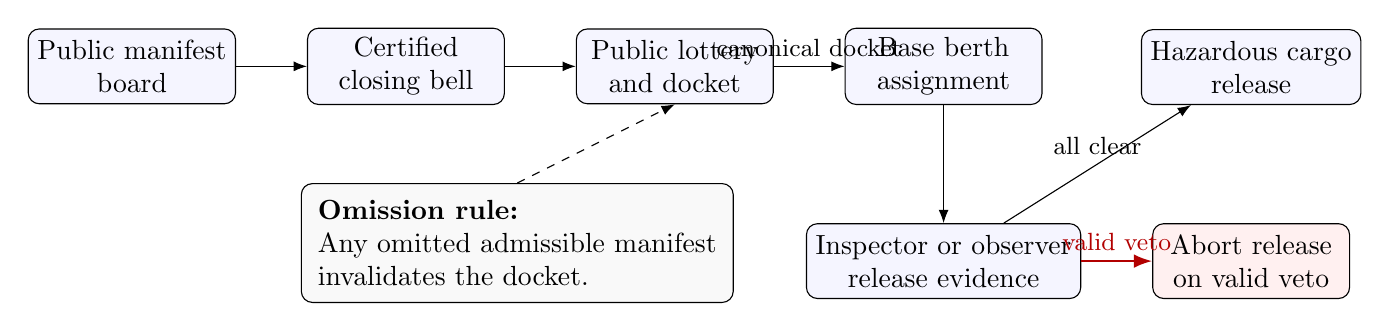
\begin{tikzpicture}[
  node distance=1.35cm and 0.9cm,
  >=Latex,
  block/.style={draw, rounded corners, align=center, minimum width=2.5cm, minimum height=0.95cm, fill=blue!4},
  abort/.style={draw, rounded corners, align=center, minimum width=2.5cm, minimum height=0.95cm, fill=red!6},
  labelbox/.style={draw, rounded corners, align=left, inner sep=6pt, fill=gray!5}
]
\node[block] (board) {Public manifest\\board};
\node[block, right=of board] (cutoff) {Certified\\closing bell};
\node[block, right=of cutoff] (lottery) {Public lottery\\and docket};
\node[block, right=of lottery] (base) {Base berth\\assignment};
\node[block, below=1.5cm of base] (sealed) {Inspector or observer\\release evidence};
\node[abort, right=of sealed] (abort) {Abort release\\on valid veto};
\node[block, above=1.5cm of abort] (release) {Hazardous cargo\\release};

\draw[->] (board) -- (cutoff);
\draw[->] (cutoff) -- (lottery);
\draw[->] (lottery) -- node[above, font=\small] {canonical docket} (base);
\draw[->] (base) -- (sealed);
\draw[->] (sealed) -- node[above, font=\small] {all clear} (release);
\draw[->, thick, red!70!black] (sealed) -- node[above, font=\small] {valid veto} (abort);

\node[labelbox, below=1.0cm of lottery, xshift=-2.0cm] (omit) {
\textbf{Omission rule:}\\
Any omitted admissible manifest\\
invalidates the docket.
};
\draw[->, dashed] (omit.north) -- (lottery.south);
\end{tikzpicture}
\caption{The thought experiment behind \AFT{}: public admission, canonical
ordering, base progress, and fail-closed release.}
\end{figure}

The correspondence is direct:

\begin{center}
\small
\begin{tabularx}{\textwidth}{>{\raggedright\arraybackslash}p{0.38\textwidth} X}
\toprule
\textbf{Port object} & \textbf{\AFT{} object} \\
\midrule
Public manifest board & Bulletin / DA surface \(B_h\) \\
Certified closing bell & Canonical cutoff \(\tau_h\) \\
Tide lottery & Public randomness beacon \(R_h\) \\
Docking docket & Canonical order \(O_h\) \\
Docket certificate & Canonical-order certificate \(OCert_h\) \\
Omitted manifest challenge & Omission proof \(\Omega(h, tx)\) \\
Base berth assignment & \code{BaseFinal} \\
Independent inspector guilds & Witness committees \\
Sampled external captains & Equal-authority observers \\
Red-flag report & Canonical observer challenge \\
Hazardous cargo release seal & \code{SealObject} under \code{SealedFinal} \\
\bottomrule
\end{tabularx}
\end{center}

This thought experiment captures the essential \AFT{} move: sparse operational
progress, dense cheap verification, objective omission, and deterministic
collapse for irreversible consequences.

\section{Protocol Family Overview}

\AFT{} is best understood as four planes that compose:

\begin{center}
\small
\begin{tabularx}{\textwidth}{>{\raggedright\arraybackslash}p{0.20\textwidth} >{\raggedright\arraybackslash}p{0.22\textwidth} >{\raggedright\arraybackslash}p{0.24\textwidth} X}
\toprule
\textbf{Plane} & \textbf{Purpose} & \textbf{Throughput-critical work} & \textbf{Authority object} \\
\midrule
Dissemination / bulletin plane & Publish the candidate transaction surface & Data dissemination and bulletin commitments & Public bulletin commitment \\
Base-finality plane & Advance the chain and commit block identity & Proposal, QC formation, guardianized certification & Validator QC + guardian certificate \\
Canonical-ordering plane & Prove the unique slot order & Succinct verification, omission dominance & \(OCert_h\) \\
Sealed-effect plane & Gate irreversible effects & Asynchronous witness / observer evidence collection & \code{SealedFinalityProof} and \code{SealObject} \\
\bottomrule
\end{tabularx}
\end{center}

The protocol modes are:

\begin{center}
\small
\begin{tabularx}{\textwidth}{>{\raggedright\arraybackslash}p{0.22\textwidth} >{\raggedright\arraybackslash}p{0.48\textwidth} X}
\toprule
\textbf{Mode} & \textbf{Role} & \textbf{Current status} \\
\midrule
\code{GuardianMajority} & Production guardian-backed base finality & Production mode \\
\code{CanonicalOrdering} & Proof-carrying equal-authority ordering & Live through \code{CommittedSurfaceV1} \\
\code{Asymptote} & Two-tier sealing and sealed-effect release & Production sealing path \\
\code{NestedGuardian} & Witness-augmented layered threshold mode & Experimental operational mode / completed theorem bridge \\
\bottomrule
\end{tabularx}
\end{center}

The key invariant is:

\[
\text{throughput-critical work} \neq \text{authority-critical work}
\]

\begin{figure}[t]
\centering
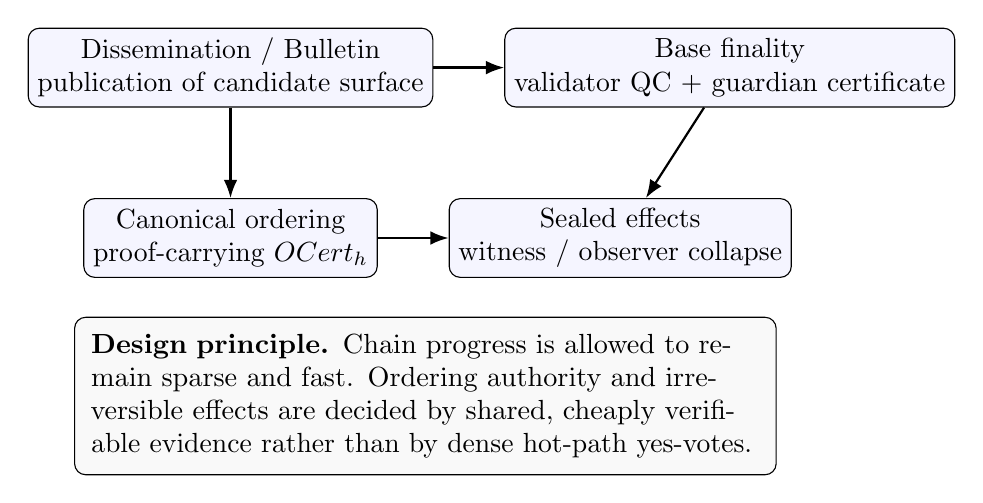
\begin{tikzpicture}[
  >=Latex,
  node distance=1.15cm and 0.9cm,
  box/.style={draw, rounded corners, align=center, minimum width=3.1cm, minimum height=1.0cm, fill=blue!4},
  note/.style={draw, rounded corners, align=left, inner sep=6pt, fill=gray!5}
]
\node[box] (bulletin) {Dissemination / Bulletin\\publication of candidate surface};
\node[box, right=of bulletin] (base) {Base finality\\validator QC + guardian certificate};
\node[box, below=of bulletin] (order) {Canonical ordering\\proof-carrying \(OCert_h\)};
\node[box, right=of order] (sealed) {Sealed effects\\witness / observer collapse};

\draw[->, thick] (bulletin) -- (base);
\draw[->, thick] (bulletin) -- (order);
\draw[->, thick] (base) -- (sealed);
\draw[->, thick] (order) -- (sealed);

\node[note, below=1.0cm of $(order)!0.5!(sealed)$, text width=0.7\textwidth] (note) {
\textbf{Design principle.}
Chain progress is allowed to remain sparse and fast.
Ordering authority and irreversible effects are decided by shared,
cheaply verifiable evidence rather than by dense hot-path yes-votes.
};
\end{tikzpicture}
\caption{\AFT{} separates publication, base progress, canonical ordering, and
sealed effect release, then recomposes them through shared evidence.}
\end{figure}

\section{System Model and Notation}
\label{sec:system-model}

\subsection{Actors}

\begin{itemize}[leftmargin=1.5em]
\item \textbf{Validator:} participates in proposal, vote, verification, and
chain execution.
\item \textbf{Guardian committee:} the registered threshold-signing committee
protecting one validator's proposal decisions.
\item \textbf{Guardian member:} an individual signer within a guardian
committee.
\item \textbf{Witness committee:} an external threshold-signing committee used
on the sealing path or in \code{NestedGuardian}.
\item \textbf{Equal-authority observer:} a validator sampled to audit a slot
under \code{Asymptote}.
\item \textbf{Registry:} the on-chain source of truth for manifests, policies,
epochs, witness sets, and verifier descriptors.
\item \textbf{Transparency log:} an append-only checkpointed evidence log for
guardian and witness statements.
\item \textbf{External verifier or gateway:} a party that checks
\code{SealObject}s and enforces replay-safe release.
\end{itemize}

\subsection{Bulletin-board time and slot model}

Consensus proceeds in heights and views. A slot is identified by
\((height, view)\). Epoch-scoped policy and committee state bind the
admissible evidence for that slot. The family should be read under a
bulletin-board recoverability model rather than a pure point-to-point timely
receipt model: safety depends on whether admissible evidence becomes publicly
retrievable by the slot cutoff, not on whether every participant receives every
message before that cutoff.

Slots are externally paced by a public cutoff object \(\tau_h\) and a public
randomness beacon \(R_h\). Honest validators that observe the same closed
public boundary derive the same ordering or sealing close-or-abort result. In
the runtime that derivation is no longer keyed off cutoff closure alone:
the bulletin plane exports a
\term{canonical bulletin-close object} binding the bulletin commitment, the
bulletin-availability certificate, and the canonical cutoff into one public
close surface. In this instantiation, positive canonical-order
publication is fail-closed at this boundary: a closed-slot order certificate is
admitted only if the published bulletin entries deterministically extract the
bulletin surface bound by the canonical bulletin-close object and the carried
bulletin-availability certificate. Universal timely receipt is not required.

Let
\[
h = \text{slot height}, \quad
v = \text{slot view},
\]
\[
B_h = \text{bulletin surface admitted before cutoff }\tau_h,
\]
\[
R_h = \text{public randomness beacon for slot }h,
\]
\[
E_h = \{tx \suchthat \mathrm{Included}(tx, B_h) \wedge \mathrm{Eligible}(tx, root_{h-1})\},
\]
\[
O_h = \mathrm{CanonicalOrder}(R_h, E_h),
\]
\[
root_h = \mathrm{Execute}(root_{h-1}, O_h).
\]

\subsection{Core assumptions}

The family-level safety claims rely on the following explicit assumptions:

\begin{itemize}[leftmargin=1.5em]
\item \textbf{Objective publication:} admitted bulletin entries, transcripts,
and challenges have stable hashes and objective inclusion paths.
\item \textbf{Verifiable bulletin availability:} the protocol exports a
bulletin-availability object, compact publication-frontier metadata that binds
the same slot surface, and a canonical bulletin-close object for each closed
ordering slot; the remaining assumption is that the underlying publication
substrate satisfies the retrieval semantics claimed by those objects. The live
runtime also requires successful closed-slot extraction before positive
canonical-order admission.
\item \textbf{Compact frontier consistency:} any carried
\code{PublicationFrontier} must bind the same-slot bulletin commitment, ordered
surface, and compact availability receipt, and same-slot conflicts or stale
predecessor links must admit short objective contradiction objects. These
frontier objects summarize the slot surface; they do not reconstruct it.
\item \textbf{Objective validity only:} theorem-critical rejection or
acceptance does not depend on private local facts.
\item \textbf{Public derivability over universal receipt:} honest validators
that observe the same closed public boundary derive the same close-or-abort
result; universal timely receipt is not required.
\item \textbf{Independent publication path:} suppressing negative evidence
requires capture of both the validator plane and the publication / registry
surface.
\item \textbf{Sealed-effect gating:} irreversible effects are released only
after surviving the canonical close-or-abort surface.
\item \textbf{Fixed epoch identities:} the validator set is epoch-scoped and
stable while the accountable rules of that epoch are enforced.
\end{itemize}

Here and throughout, ``ordinary permissioned setting'' means fixed
authenticated authorities, deterministic local verification, public
hash-addressed protocol objects, epoch-scoped identity state, and eventual-
fair delivery and persistence of admissible protocol artifacts, with no
trusted relay, privileged coordinator, TEE, theorem-side bootstrap oracle, or
hidden external recovery service.
Fixed authenticated membership is part of the theorem statement, not a missing
crutch. The hidden-helper exclusions are relay, coordinator, TEE, bootstrap
oracle, and external recovery service --- not epoch-scoped authenticated
identity itself.

\subsection{Evidence objects}

The family-level evidence objects are:

\begin{itemize}[leftmargin=1.5em]
\item validator quorum certificates over block proposals,
\item guardian quorum certificates over slot decisions,
\item witness certificates over guardianized slots,
\item canonical-order certificates over bulletin surfaces,
\item omission proofs over ordered-set incompleteness,
\item observer transcripts, observer challenges, and canonical close-or-abort
objects over sealed finality,
\item sealed-effect proof objects with replay-safe nullifiers.
\end{itemize}

All honest nodes are required to derive the same acceptance result from the
same admissible evidence set.

\subsection{Accountable publication rules}

Objective AFT faults are not merely audit artifacts. In the runtime they
are first-class accountable protocol objects:

\begin{itemize}[leftmargin=1.5em]
\item \code{OmissionProof} names the validator accountable for the dominated
positive order object.
\item \code{AsymptoteObserverChallenge} determines accountability by kind:
\code{MissingTranscript} and \code{ConflictingTranscript} blame the assigned
observer; \code{TranscriptMismatch}, \code{VetoTranscriptPresent}, and
\code{InvalidCanonicalClose} blame the producer / positive-close path.
\item Valid objective fault evidence is replay-deduplicated on chain.
\item Policy-controlled membership updates are aftermath only: the same
evidence may trigger best-effort immediate quarantine and stage next-epoch
eviction, but the decisive negative object remains valid even when those
membership updates are disabled, delayed, or skipped.
\end{itemize}

These rules do not change the hot path. They strengthen the adversary model:
arbitrary behavior is tolerated only insofar as it remains publicly revealable
and penalty-bearing.

\section{Public State Continuity with Extractable Obstructions}
\label{sec:psc}

\AFT{}'s deeper theorem target is not a new round gadget. It is a new source of
uniqueness. Classical Byzantine agreement derives uniqueness from overlap of
dense positive quorums. \AFT{} instead seeks a rigidity theorem over public slot
objects: once the slot boundary is closed, the space of admissible public
continuations should collapse to one canonical object or one canonical abort.

\subsection{Boundary-conditioned execution language}

For a closed slot boundary define
\[
\partial_h := (root_{h-1}, \beta_h, \tau_h, R_h, p_h),
\]
where \(\beta_h\) is the canonical bulletin-close object binding the bulletin
commitment, bulletin-availability certificate, and canonical cutoff whose
recoverable surface is \(B_h\); \(\tau_h\) is the canonical cutoff object;
\(R_h\) is the slot randomness beacon; and \(p_h\) is the policy descriptor
governing admissible checks for slot \(h\).

Let a \term{public execution object} for slot \(h\) be a normalized public
codeword
\[
X_h := (B_h, E_h, O_h, root_h, \sigma_h),
\]
where \(E_h\) is the eligible subset, \(O_h\) is the canonical ordered object,
\(root_h\) is the resulting state commitment, and \(\sigma_h\) is the
slot-local sealing surface needed to determine whether the slot closes or
aborts. The important point is that \(X_h\) is not a distributed transcript.
It is the public quotient of the slot after irrelevant schedule variation is
factored out.

Define the boundary-conditioned language
\[
\mathcal{L}(\partial_h) := \{X \suchthat \exists \pi \; \mathrm{Accept}(\partial_h, X, \pi)=1 \}.
\]

Here \(\pi\) is a succinct admissibility witness. For canonical ordering,
\(\pi\) is the proof-carrying order certificate witness. For deterministic
observer sealing, \(\pi\) is the witness that the canonical transcript surface,
challenge surface, and close-or-abort object satisfy the slot policy.

\subsection{Obstruction extractability}

The companion rejection relation is
\[
\mathrm{Reject}(\partial_h, Y, \omega)=1,
\]
where \(Y\) is a fully specified candidate public execution object and
\(\omega\) is a short public objective contradiction witness.

\AFT{} seeks \term{obstruction-complete local testability}: for a fixed closed
boundary, every fully specified candidate lies in exactly one of two states,
\[
\Big(\exists \pi \; \mathrm{Accept}(\partial_h, Y, \pi)=1\Big)
\;\oplus\;
\Big(\exists \omega \; \mathrm{Reject}(\partial_h, Y, \omega)=1\Big).
\]

This xor formulation is the software-only analogue of state continuity. It is
stronger than merely having a valid proof system. It says every non-admissible
candidate exposes a short public contradiction witness.

In the live repository, the obstruction basis is not abstract:

\begin{itemize}[leftmargin=1.5em]
\item ordering uses a first-class canonical abort taxonomy over the canonical
bulletin surface: missing certificates, bulletin-surface reconstruction
failures, bulletin-surface mismatches, invalid bulletin-close formation,
omission-dominated candidates, certificate-height mismatches, randomness
mismatches, ordered-transactions-root mismatches, resulting-state-root
mismatches, invalid public-input bindings, invalid bulletin-availability
bindings, and invalid proof bindings,
\item deterministic observer sealing uses objective challenge kinds over the
canonical transcript and challenge surface,
\item the accountable-adversary layer turns those same objects into
penalty-bearing public fault evidence.
\end{itemize}

\subsection{Unique collapse object}

The slot should not merely admit at most one positive object. It should admit
at most one \term{collapse object}:
\[
\mathrm{Collapse}(\partial_h) \in \{\mathrm{Close}(X_h), \mathrm{Abort}(\Omega_h)\}.
\]

Here \(\mathrm{Close}(X_h)\) denotes the unique admissible positive object when
the obstruction surface is empty, while \(\mathrm{Abort}(\Omega_h)\) denotes
the unique negative object induced by a non-empty valid obstruction surface.
Negative evidence does not create a second truth. It forces the slot to land on
its canonical abort object instead of a close object.

In the runtime this collapse object is not merely an abstract proof
target. Validator finalization publishes a first-class
\code{CanonicalCollapseObject} through \code{guardian\_registry}, and later
consensus verification cross-checks any published copy against the same
proof-carried ordering and sealing surface when parent-state data is available.
In the current recursive-continuity slice, \code{CanonicalCollapseObject}
also carries a rolling \code{previous\_canonical\_collapse\_commitment\_hash}, and in the
current clean-break runtime slice it also carries
\code{continuity\_accumulator\_hash} together with
\code{continuity\_recursive\_proof}, so the current slot's collapse object is
linked to the previously persisted or published collapse object rather than
standing as an isolated per-slot fact. The newest proposal-surface slice
pushes that same predecessor link into the signed header itself:
\code{BlockHeader} now carries
\code{previous\_canonical\_collapse\_commitment\_hash} in
its signed preimage and also carries a typed
\code{CanonicalCollapseExtensionCertificate}. That certificate now carries the
predecessor commitment plus the predecessor recursive-proof hash, while the
public predecessor \code{CanonicalCollapseObject} now carries only a single
recursive proof step rather than a carried predecessor-proof tree. Each
recursive proof step still binds a predecessor collapse commitment,
predecessor commitment hash, predecessor payload hash, and previous proof
hash; the rolling
\code{continuity\_accumulator\_hash} remains in place as the companion
accumulator over the same chain. The implementation surface
distinguishes the reference \code{HashPcdV1} carrier from a backend slot
\code{SuccinctSp1V1}, and the runtime exposes a dedicated continuity-verifier
seam for those recursive public inputs via \code{ioi-api} and
\code{zk-driver-succinct}. That seam is now wired into the live protocol:
\code{GuardianMajority} invokes it while validating proposal and QC continuity
for carried or anchored \code{SuccinctSp1V1} proof steps, and validator
durable-state checks invoke the same backend before a persisted
\code{CanonicalCollapseObject} is treated as authoritative. Proposal verification checks that the carried
predecessor commitment hash matches the signed predecessor link, checks that
the predecessor commitment's resulting state root matches the signed parent-state root, and
checks that the carried predecessor proof hash matches the anchored
predecessor collapse object already persisted or published in protocol state.
Leaders in
\code{Asymptote} stall rather than propose when the required extension
certificate or anchored predecessor collapse object is unavailable, proposal
verification rechecks that implied predecessor commitment against both the
signed predecessor commitment link and the parent-state root, checks the
carried predecessor proof hash against the anchored predecessor proof on the
public collapse object, and QC progression only treats continuity-linked headers as
progress-authoritative.

\begin{theorem}[Public State Continuity with Extractable Obstructions]
Assume a closed boundary \(\partial_h\), objective publication, a
protocol-native retrievability plane, compact publication-frontier consistency,
objective validity only, and proof soundness. Then the instantiated and
normative theorem shape
for \AFT{} is:
\begin{enumerate}[leftmargin=1.5em]
\item \(\mathcal{L}(\partial_h)\) contains at most one admissible public
execution object,
\item every fully specified candidate \(Y \notin \mathcal{L}(\partial_h)\)
admits a short public objective obstruction witness \(\omega\) such that
\(\mathrm{Reject}(\partial_h, Y, \omega)=1\),
\item therefore the slot admits at most one admissible collapse object, either
the unique close object or the unique abort object.
\end{enumerate}
\end{theorem}

This theorem is the precise form of the software-only continuity primitive that
the instantiated \AFT{} runtime realizes. The later ordering, collapse,
recovery, restart, and sealed-effect sections are concrete theorem instances
and composition layers of this same continuity statement, not separate
aspirations. It does not claim that the classical DLS / PBFT frontier
disappeared inside the standard dense-vote model. The point is different: the
uniqueness source has moved from quorum overlap into the public-evidence
language itself.
In the instantiated runtime, compact publication frontiers internalize same-slot and
predecessor consistency inside the live protocol, while the protocol-native
retrievability plane discharges closed-bulletin extraction-or-abort on the
cold path.

\subsection{Lemma program}

The clean proof path is a filtration rather than a single opaque argument:
\[
\mathcal{L}_0(\partial_h) \supseteq \mathcal{L}_1(\partial_h) \supseteq \cdots
\supseteq \mathcal{L}_k(\partial_h),
\]
where each refinement adds one structural constraint and each failed refinement
admits a short witness.

The repository's theorem program is:

\begin{enumerate}[leftmargin=1.5em]
\item \textbf{Boundary Fixing Lemma.} The closed boundary fixes the admissible
publication domain.
\item \textbf{Bulletin Close Lemma.} The canonical bulletin-close object fixes
the unique recoverable bulletin surface for the slot.
\item \textbf{Eligibility Determinism Lemma.} The predecessor commitment and
boundary fix the eligible subset.
\item \textbf{Order Determinism Lemma.} The boundary and eligible subset fix
the canonical ordered object.
\item \textbf{Transition Determinism Lemma.} The ordered object fixes the next
state commitment.
\item \textbf{Collapse Exclusivity Lemma.} A slot cannot admit both a canonical
close object and a canonical abort object.
\item \textbf{Obstruction Soundness Lemma.} Every valid omission proof or
observer challenge objectively rejects its target candidate.
\item \textbf{Obstruction Completeness Lemma.} Every invalid fully specified
candidate contains at least one minimal public obstruction witness.
\item \textbf{Extractor Sufficiency Lemma.} Given the canonical bulletin-close
object, any honest validator can run the protocol-defined bulletin extractor to
reconstruct the same bulletin surface; in this instantiation, admission
of the positive ordering object already requires this extraction to succeed
over the published closed-slot surface. One honest validator remains sufficient
to surface the resulting positive or negative object under the instantiated runtime
model.
\end{enumerate}

One honest validator is surfacing-sufficient but never trust-bearing:
correctness does not attach to the revealer's identity, because any honest
validator observing the same closed boundary derives the same decisive object.

The theorem surfaces of this paper are instances of that program:

\begin{itemize}[leftmargin=1.5em]
\item \code{CanonicalOrdering} instantiates unique admissibility and
extractable obstruction through proof-carrying order certificates plus omission
dominance.
\item \code{Asymptote} instantiates unique collapse through canonical
transcript/challenge surfaces plus close-or-abort exclusivity.
\end{itemize}

\section{The \AFT{} Deterministic Base Engine}

\AFT{} modes share a deterministic core engine for proposal flow, QC
formation, locking, and view progression.

\subsection{Deterministic leadership and view progression}

For a given height and view, the implementation selects the proposer by
deterministic round-robin over the active validator set:

\[
\mathrm{leader}(h, v) = V_h[(h - 1 + v) \bmod |V_h|].
\]

Here \(V_h\) is the active validator set for height \(h\) after operational
quarantine filters are applied.

View \(0\) proposals do not carry a timeout certificate. Any non-zero view
proposal must carry a valid timeout certificate for the previous unsuccessful
view. The pacemaker advances views monotonically and resets timers on observed
progress.

\subsection{Validator quorum certificates}

In \code{GuardianMajority}, \code{Asymptote}, and \code{NestedGuardian},
validator quorum is a strict simple majority of active validator weight, not a
classical \(2/3 + 1\) quorum:

\[
\mathrm{QCQuorum}(V_h) > \frac{1}{2}\mathrm{Weight}(V_h).
\]

This is safe only because the validator quorum is \emph{not} the sole
authority object. A proposal must also satisfy guardian-layer admissibility.

Timeout certificates use the same simple-majority rule over view-change votes.

\subsection{Locking, 2-chain commit, and divergence guard}

Validators maintain a lock on the highest safe parent QC they have observed. A
validator votes only when the proposal extends the lock or is in a strictly
higher view than the lock.

Base commitment uses a 2-chain rule:

\begin{itemize}[leftmargin=1.5em]
\item let \(QC_{parent}\) certify parent block \(P\),
\item let \(QC_{child}\) certify child block \(C\),
\item if \(C\) directly extends \(P\) and the views are consecutive, then
\(P\) becomes a pending commit.
\end{itemize}

The implementation delays final durability by a guard window
\(\Delta_{guard}\) before a pending commit is released. The purpose of the
guard window is operational, not purely algebraic: it gives divergence
evidence or panic signals time to propagate before a conflicting branch is
treated as durable.

This produces a fail-closed operational behavior:

\begin{itemize}[leftmargin=1.5em]
\item sparse chain progress happens on the hot path,
\item conflicting evidence is surfaced before irreversible consequences,
\item divergence proofs quarantine the affected node rather than silently
allowing fork continuation.
\end{itemize}

\section{GuardianMajority: Production Base Finality}

\code{GuardianMajority} is the production fault model for \AFT{} base finality.
Validator votes alone never make a proposal admissible. Every valid proposal
must also carry a guardian committee certificate that verifies against current
registered committee state.

\subsection{Guardian certificate object}

The guardian certificate binds:

\begin{itemize}[leftmargin=1.5em]
\item the guardian committee manifest hash,
\item the active epoch,
\item the canonical decision hash for the slot payload,
\item a monotonic guardian counter,
\item a guardian trace root,
\item a measurement root,
\item the signer bitfield,
\item the aggregated BLS signature,
\item a transparency-log checkpoint,
\item and, in \code{NestedGuardian}, an optional experimental witness
certificate.
\end{itemize}

The guardian decision payload is slot-scoped. Honest guardians are assumed not
to sign two different decisions for the same slot.

\subsection{Verification rule}

A guardianized proposal is admissible only if all of the following hold:

\begin{enumerate}[leftmargin=1.5em]
\item the referenced guardian committee manifest is registered on-chain for the
active epoch,
\item the certificate manifest hash matches the registered manifest,
\item the certificate epoch matches the manifest epoch and current epoch,
\item the decision hash matches the slot's canonical guardian decision payload,
\item the measurement root matches the decision payload,
\item the signer set is valid, unique, and meets the committee threshold,
\item the aggregated signature verifies against the manifest public keys,
\item the attached transparency-log checkpoint verifies against the anchored
log descriptor and append-only proof.
\end{enumerate}

The transparency log is an accountability layer. It does not replace threshold
safety. It makes issued decisions, checkpoints, and later slashing evidence
publicly checkable.

\subsection{Committee threshold model}

Let a guardian committee have threshold \(t\) and size \(n\). Conflicting slot
certificates require enough equivocators to cover the minimum quorum
intersection:

\[
f < 2t - n.
\]

Production committees therefore use strict majority thresholds:

\[
t = \left\lfloor \frac{n}{2} \right\rfloor + 1.
\]

This guarantees pairwise quorum intersection. It also exposes an important
operational nuance:

\begin{itemize}[leftmargin=1.5em]
\item odd-sized simple-majority committees tolerate zero equivocating guardian
members at the committee layer,
\item even-sized majority committees tolerate one equivocator before threshold
intersection is exhausted.
\end{itemize}

Production safety therefore relies on both threshold intersection and stronger
guardian non-equivocation guarantees.

\subsection{Safety statement}

\begin{proposition}[GuardianMajority Safety]
No two conflicting blocks can both finalize for the same \((height, view)\) if
guardian committee manifests are current, committee thresholds are majority
thresholds, honest guardians do not equivocate for the same slot,
transparency-log checkpoints and registry state are current enough to verify
admissibility, and validators finalize only guardian-admissible blocks.
\end{proposition}

This is not a classical \(3f + 1\) theorem. It is a composed threshold theorem
over validators, guardians, registry state, and shared evidence. That
statement is local to the guardian-backed base-finality layer. It does not
delimit the paper's promoted theorem surface. The promoted durable-agreement
claim is carried by the later proof-carrying close-or-abort and canonical-
collapse architecture, which is precisely why the classical \(3f + 1\)
threshold is not load-bearing there.

\subsection{Liveness model}

Liveness is secondary to safety. Progress requires:

\begin{itemize}[leftmargin=1.5em]
\item enough active validators to form the simple-majority validator QC,
\item enough guardian members to satisfy the committee threshold,
\item current registry state for the epoch,
\item current enough checkpoint and log availability.
\end{itemize}

If these degrade, the protocol prefers stalling over accepting unsafe evidence.

\section{Canonical Ordering}

\code{CanonicalOrdering} is the proof-carrying ordering path that gives
\AFT{} its \code{99\%} equal-authority ordering consensus claim.

\subsection{Objective}

For each slot \(h\), define a unique canonical ordered set \(O_h\) and a
certificate \(OCert_h\) such that:

\begin{itemize}[leftmargin=1.5em]
\item every honest verifier can check \(OCert_h\) cheaply,
\item any omission is objectively provable,
\item the ordered set is recoverable from public data,
\item the live hot path carries a compact publication frontier that binds the
same-slot bulletin / ordering / availability surface and predecessor
continuity,
\item conflicting valid certificates for the same slot are impossible,
\item arbitrary behavior by almost all validators cannot create a conflicting
valid ordering outcome because the closed bulletin boundary admits one
deterministically derivable close-or-abort result.
\end{itemize}

\subsection{Canonical objects}

For slot \(h\),
\[
B_h = \text{bulletin surface admitted before }\tau_h,
\]
\[
R_h = \text{public randomness beacon for slot }h,
\]
\[
E_h = \{tx \suchthat \mathrm{Included}(tx, B_h) \wedge \mathrm{Eligible}(tx, root_{h-1})\},
\]
\[
O_h = \mathrm{CanonicalOrder}(R_h, E_h),
\]
\[
root_h = \mathrm{Execute}(root_{h-1}, O_h).
\]

The abstract certificate is
\[
OCert_h =
\left(
  h,
  root_{h-1},
  cutoff_h,
  bulletin\_commitment_h,
  ordered\_commitment_h,
  root_h,
  witness_h
\right).
\]

\subsection{Bulletin, cutoff, and admissibility assumptions}

The ordering theorem is conditional on the following named assumptions.

\paragraph{A1. Objective publication.}
Each admitted transaction or batch in \(B_h\) has a stable content hash, a
verifiable inclusion path into the bulletin commitment, and an objective
publication time or publication position relative to the slot cutoff.

\paragraph{A2. Endogenous retrievability.}
The bulletin contents committed by \(bulletin\_commitment_h\) are reconstructed
or deterministically aborted from protocol-native retrievability objects rooted
in the canonical bulletin close for slot \(h\). Compact publication-frontier
summaries and availability certificates bind that claim on the hot path, while
retrievability profiles, shard manifests, custody assignments, custody
receipts, custody responses, and objective challenge objects close the
extraction-or-abort loop on the cold path.
Without that plane, uniqueness may still hold while timely materialization of
the same close-or-abort surface can fail.

\paragraph{A3. Append-only or equivocation-evident commitment.}
The bulletin commitment and any carried publication frontier for slot \(h\)
must be append-only or otherwise make same-slot equivocation or stale
predecessor linkage objectively detectable at the slot boundary.

\paragraph{A4. Eligibility determinism.}
\(\mathrm{Eligible}(tx, root_{h-1})\) is deterministic and locally checkable
from the committed predecessor root and the transaction object. Honest
validators therefore derive the same eligible set \(E_h\) from the same public
inputs.

\paragraph{A5. Proof soundness.}
\(\mathrm{VerifyProof}(witness_h) = \mathrm{true}\) implies that the witness
obligations for cutoff binding, bulletin binding, ordering, state transition,
retrievability commitments, and omission commitments actually hold.

The cutoff \(\tau_h\) is not a private local clock read. It is a protocol-bound
object. In the instantiated runtime, the cutoff is bound directly into
the published bulletin commitment and into the canonical public-input set.
Eligibility is deterministic with respect to the predecessor state root and the
transaction object. This prevents local reinterpretation of the eligible set.

\subsection{Current runtime instantiation}

The runtime surfaces the abstract objects above as the following concrete
objects:

\begin{center}
\scriptsize
\begin{tabularx}{\textwidth}{>{\raggedright\arraybackslash}p{0.32\textwidth} X}
\toprule
\textbf{Runtime object} & \textbf{Current fields} \\
\midrule
\code{BulletinCommitment} & \code{(height, cutoff\_timestamp\_ms, bulletin\_root, entry\_count)} \\
\code{BulletinSurfaceEntry} & \code{(height, tx\_hash)} \\
\shortstack[l]{\code{BulletinAvailability}\\\code{Certificate}} & \code{(height, bulletin\_commitment\_hash, recoverability\_root)} \\
\code{BulletinRetrievabilityProfile} & \shortstack[l]{\code{(height, bulletin\_commitment\_hash,}\\\code{bulletin\_availability\_certificate\_hash, recoverability\_root,}\\\code{shard\_count, recovery\_threshold, custody\_threshold)}} \\
\code{BulletinShardManifest} & \shortstack[l]{\code{(height, bulletin\_commitment\_hash,}\\\code{bulletin\_availability\_certificate\_hash,}\\\code{bulletin\_retrievability\_profile\_hash, recoverability\_root,}\\\code{entry\_count, shard\_count, recovery\_threshold, shard\_commitment\_root)}} \\
\code{BulletinCustodyAssignment} & \shortstack[l]{\code{(height, bulletin\_retrievability\_profile\_hash,}\\\code{bulletin\_shard\_manifest\_hash, validator\_set\_commitment\_hash,}\\\code{assignments)}} \\
\code{BulletinCustodyReceipt} & \shortstack[l]{\code{(height, bulletin\_commitment\_hash,}\\\code{bulletin\_availability\_certificate\_hash,}\\\code{bulletin\_retrievability\_profile\_hash, bulletin\_shard\_manifest\_hash,}\\\code{custodian\_count, custody\_threshold, custody\_root)}} \\
\code{BulletinCustodyResponse} & \shortstack[l]{\code{(height, bulletin\_commitment\_hash,}\\\code{bulletin\_availability\_certificate\_hash,}\\\code{bulletin\_retrievability\_profile\_hash, bulletin\_shard\_manifest\_hash,}\\\code{bulletin\_custody\_assignment\_hash, bulletin\_custody\_receipt\_hash,}\\\code{served\_shards)}} \\
\code{BulletinRetrievabilityChallenge} & \shortstack[l]{\code{(height, kind, bulletin\_commitment\_hash,}\\\code{bulletin\_availability\_certificate\_hash,}\\\code{bulletin\_retrievability\_profile\_hash, bulletin\_shard\_manifest\_hash,}\\\code{bulletin\_custody\_assignment\_hash, bulletin\_custody\_receipt\_hash,}\\\code{bulletin\_custody\_response\_hash, details)}} \\
\code{BulletinReconstructionCertificate} & \shortstack[l]{\code{(height, bulletin\_commitment\_hash,}\\\code{bulletin\_availability\_certificate\_hash,}\\\code{bulletin\_retrievability\_profile\_hash, bulletin\_shard\_manifest\_hash,}\\\code{bulletin\_custody\_assignment\_hash, bulletin\_custody\_receipt\_hash,}\\\code{bulletin\_custody\_response\_hash, canonical\_bulletin\_close\_hash,}\\\code{canonical\_order\_certificate\_hash, reconstructed\_entry\_count,}\\\code{reconstructed\_bulletin\_root)}} \\
\code{BulletinReconstructionAbort} & \shortstack[l]{\code{(height, kind, bulletin\_commitment\_hash,}\\\code{bulletin\_availability\_certificate\_hash,}\\\code{bulletin\_retrievability\_profile\_hash, bulletin\_shard\_manifest\_hash,}\\\code{bulletin\_custody\_receipt\_hash, bulletin\_retrievability\_challenge\_hash,}\\\code{canonical\_order\_abort\_hash, details)}} \\
\code{PublicationAvailabilityReceipt} & \shortstack[l]{\code{(height, bulletin\_commitment\_hash,}\\\code{ordered\_transactions\_root\_hash, resulting\_state\_root\_hash,}\\\code{receipt\_root)}} \\
\code{PublicationFrontier} & \shortstack[l]{\code{(height, view, counter, parent\_frontier\_hash,}\\\code{bulletin\_commitment\_hash, ordered\_transactions\_root\_hash,}\\\code{availability\_receipt\_hash)}} \\
\code{PublicationFrontierContradiction} & \code{(height, kind, candidate\_frontier, reference\_frontier)} \\
\shortstack[l]{\code{CanonicalBulletin}\\\code{Close}} & \shortstack[l]{\code{(height, cutoff\_timestamp\_ms, bulletin\_commitment\_hash,}\\\code{bulletin\_availability\_certificate\_hash,}\\\code{bulletin\_retrievability\_profile\_hash, bulletin\_shard\_manifest\_hash,}\\\code{bulletin\_custody\_receipt\_hash, entry\_count)}} \\
\shortstack[l]{\code{CanonicalOrder}\\\code{PublicInputs}} & \shortstack[l]{\code{(height, parent\_state\_root\_hash, bulletin\_commitment\_hash,}\\\code{randomness\_beacon, ordered\_transactions\_root\_hash,}\\\code{resulting\_state\_root\_hash, cutoff\_timestamp\_ms)}} \\
\code{CanonicalOrderProofSystem} & concrete variants \code{HashBindingV1} and \code{CommittedSurfaceV1} \\
\shortstack[l]{\code{CommittedSurface}\\\code{CanonicalOrderProof}} & \code{(recoverability\_root, omission\_commitment\_root)} \\
\shortstack[l]{\code{CanonicalOrder}\\\code{Certificate}} & \shortstack[l]{\code{(height, bulletin\_commitment, bulletin\_availability\_certificate,}\\\code{randomness\_beacon, ordered\_transactions\_root\_hash,}\\\code{resulting\_state\_root\_hash, proof, omission\_proofs)}} \\
\shortstack[l]{\code{CanonicalOrder}\\\code{PublicationBundle}} & \shortstack[l]{\code{(bulletin\_commitment, bulletin\_entries, bulletin\_availability\_certificate,}\\\code{bulletin\_retrievability\_profile, bulletin\_shard\_manifest,}\\\code{bulletin\_custody\_receipt, canonical\_order\_certificate)}} \\
\shortstack[l]{\code{CanonicalOrder}\\\code{Abort}} & \shortstack[l]{\code{(height, reason, details, bulletin\_commitment\_hash,}\\\code{bulletin\_availability\_certificate\_hash, bulletin\_close\_hash,}\\\code{canonical\_order\_certificate\_hash)}} \\
\bottomrule
\end{tabularx}
\end{center}

\code{HashBindingV1} is the reference verifier family: its proof bytes are a
canonical hash binding over the public-input hash. \code{CommittedSurfaceV1}
is the live proof family: its proof payload contains the recoverability root
and the omission-commitment root for the committed surface. In the current
runtime, positive ordering artifacts are published through the atomic
\code{CanonicalOrderPublicationBundle}, carrying the bound retrievability
profile / manifest / custody-receipt objects, while the registry
deterministically materializes the coupled custody-assignment and
custody-response objects over the same slot surface before admitting the
positive lane. Positive committed
blocks also carry a compact signed \code{PublicationFrontier}: it binds the
same-slot bulletin commitment, ordered-transactions root, and compact
publication-availability receipt, and it hash-links that summary to the
previous slot's frontier. Short \code{PublicationFrontierContradiction}
objects make same-slot conflict or stale predecessor linkage objectively
rejectable on the hot path. Those frontier objects internalize compact
publication consistency, but they do not replace the protocol-native
retrievability plane that reconstructs or aborts the full bulletin surface.
Validators also run a block-local derivation pass over
the committed block boundary: they derive either a
\code{CanonicalOrderExecutionObject} or a \code{CanonicalOrderAbort}, and
publish the abort artifact when the proof-carried positive object cannot be
derived. When the endogenous retrievability lane succeeds, the registry
materializes a first-class \code{BulletinReconstructionCertificate} bound to
the canonical close, canonical-order certificate, and the same retrievability
objects. When endogenous retrievability evidence dominates that same surface,
the registry also materializes a specialized
\code{BulletinReconstructionAbort} object bound to the challenge and the paired
\code{CanonicalOrderAbort}, so reconstruction-impossible failure is named as a
first-class protocol object rather than only as a generic ordering abort.

\subsection{Acceptance rule}

Every validator applies the same deterministic rule:

\[
\begin{aligned}
\mathrm{Accept}(OCert_h)
\iff\;& \mathrm{VerifyProof}(witness_h) \\
&\wedge \mathrm{VerifyCutoff}(cutoff_h) \\
&\wedge \mathrm{PredecessorAccepted}(root_{h-1}) \\
&\wedge \neg \exists tx : \mathrm{ValidOmission}(h, tx).
\end{aligned}
\]

In the implementation this specializes to:

\begin{itemize}[leftmargin=1.5em]
\item the certificate height and bulletin height must match the block height,
\item the randomness beacon must match the slot schedule,
\item the bulletin commitment must match the published bulletin when that
bulletin is available from anchored state,
\item any carried \code{PublicationFrontier} must match the same-slot bulletin
commitment, ordered-transactions root, and publication-availability receipt
hash,
\item when a predecessor frontier exists, the carried
\code{PublicationFrontier} must extend it by counter and parent hash,
\item no published \code{PublicationFrontierContradiction} may already dominate
the slot,
\item positive canonical-order admission in the runtime additionally
requires successful closed-slot extraction over the published bulletin entries,
the carried bulletin-availability certificate, and the canonical
bulletin-close object,
\item the ordered-transactions root and resulting state root must match the
block header,
\item the proof must match the canonical public inputs,
\item the recoverability root must match the certificate commitments,
\item the omission-commitment root must match the omission-proof set.
\end{itemize}

If the omission-proof set is non-empty, the candidate certificate is rejected
immediately.

No dense positive vote on the order is required once a valid \(OCert_h\) is
surfaced. The current verifier entry point for this rule is
\code{verify\_canonical\_order\_certificate}.

\subsection{Omission dominance}

An omission is objective when a transaction:

\begin{itemize}[leftmargin=1.5em]
\item was included in \(B_h\) before \(\tau_h\),
\item was eligible under \(root_{h-1}\),
\item and is absent from the committed ordered set \(O_h\).
\end{itemize}

Define the omission proof
\[
\Omega(h, tx) =
\left(
\begin{array}{l}
  inclusion\_proof(tx, bulletin_h), \\
  cutoff\_admissibility\_proof(tx, cutoff_h), \\
  eligibility\_proof(tx, root_{h-1}), \\
  nonmembership\_proof(tx, O_h)
\end{array}
\right).
\]

Its semantics are:
\[
\mathrm{Valid}(\Omega(h, tx)) \Rightarrow \mathrm{Reject}(OCert_h).
\]

This is the central \AFT{} ordering move. A candidate does not need to win a
dense round of positive endorsements if any incomplete view can be killed
objectively.

Omission dominance is a correctness rule, not a punishment rule. A valid
omission proof kills the candidate immediately whether or not slashing,
quarantine, or next-epoch removal ever fires.

\subsection{Uniqueness, publication frontiers, and recoverability}

\begin{theorem}[Uniqueness]
If \(\mathrm{ValidOrderCert}(h, C_1)\) and \(\mathrm{ValidOrderCert}(h, C_2)\),
then \(C_1\) and \(C_2\) commit the same canonical ordered set \(O_h\).
\end{theorem}

The reason is structural:

\begin{itemize}[leftmargin=1.5em]
\item the predecessor root is fixed,
\item the cutoff object is canonical,
\item the bulletin commitment is canonical,
\item eligibility is deterministic,
\item the ordering function is deterministic,
\item proof soundness forbids a witness for a different ordered set.
\end{itemize}

The live publication-frontier slice sits between uniqueness and
recoverability. A frontier gives a compact signed summary of the claimed
bulletin / ordering surface and its predecessor link, so same-slot conflict or
stale lineage is objectively rejectable without reconstructing the full
bulletin on the hot path. But the frontier only binds hashes and receipt roots;
it is not itself the recoverable bulletin surface.

\begin{theorem}[Endogenous Retrievability]
If \(\mathrm{ValidOrderCert}(h, C)\) and the canonical bulletin close plus
protocol-native retrievability plane for slot \(h\) are present and
unchallenged, then every honest verifier can reconstruct the same ordered set
\(O_h\) from protocol objects alone: the canonical close, bound frontier /
availability commitments, retrievability profile, shard manifest, custody
receipt, positive reconstruction certificate, and published bulletin entries.
\end{theorem}

Endogenous retrievability matters because the accepted order is not merely
unique. The compact frontier tells validators which surface is being claimed;
the retrievability plane tells them that the full surface can actually be
reconstructed or objectively aborted from protocol evidence.

The hot path and the cold path do not carry different truths. The frontier
binds the claimed surface compactly; the retrievability plane reconstructs or
objectively aborts that same surface; both terminate on the same canonical
close-or-abort object.

\subsection{\texorpdfstring{\(99\%\)}{99\%} equal-authority ordering consensus}

\AFT{}'s ordering claim is a proof-carrying consensus theorem whose decisive
object is revealed rather than manufactured by dense positive yes-votes.
Revelation is not a weaker post hoc reporting layer here; it is the equal-
authority surfacing mechanism for the uniquely valid public execution object
already fixed by the closed public boundary.

\begin{theorem}[99\% Equal-Authority Ordering Consensus]
Assume:
\begin{enumerate}[leftmargin=1.5em]
\item the closed bulletin surface \(B_h\) bound by the carried publication
frontier and bulletin commitment is governed by a canonical bulletin close and
protocol-native retrievability plane that deterministically yields extraction
or abort,
\item the cutoff object for slot \(h\) is canonical,
\item bulletin commitments, compact publication-frontier bindings, and omission
proofs are objectively verifiable,
\item same-slot frontier conflicts and stale predecessor links admit short
objective contradiction objects,
\item the proof system is sound.
\end{enumerate}
Then even if \(99\%\) of validators behave arbitrarily, they cannot create a
conflicting valid canonical-order outcome for slot \(h\). More strongly,
every honest validator that observes the same closed ordering boundary derives
the same positive order object or omission-dominated abort.
\end{theorem}

Compact publication frontiers therefore internalize cheap same-slot and
predecessor consistency checks on the live path, while recoverability remains
the stronger assumption needed to turn that compact claim into a publicly
reconstructable ordered set.

\begin{figure}[t]
\centering
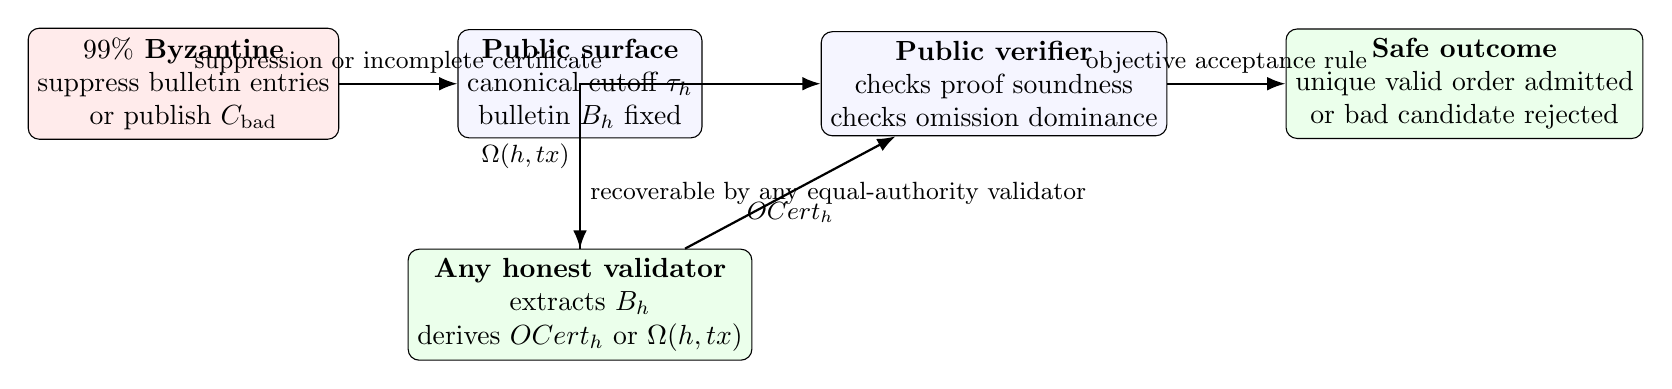
\begin{tikzpicture}[
  >=Latex,
  node distance=1.4cm and 1.5cm,
  stage/.style={draw, rounded corners, minimum width=3.05cm, minimum height=1.15cm, align=center, fill=blue!4},
  bad/.style={draw, rounded corners, minimum width=3.05cm, minimum height=1.15cm, align=center, fill=red!8},
  good/.style={draw, rounded corners, minimum width=3.05cm, minimum height=1.15cm, align=center, fill=green!8},
  note/.style={font=\small, align=center}
]
\node[bad] (attackers) {\textbf{\(99\%\) Byzantine}\\suppress bulletin entries\\or publish \(C_{\mathrm{bad}}\)};
\node[stage, right=of attackers] (bulletin) {\textbf{Public surface}\\canonical cutoff \(\tau_h\)\\bulletin \(B_h\) fixed};
\node[good, below=of bulletin] (recoverer) {\textbf{Any honest validator}\\extracts \(B_h\)\\derives \(OCert_h\) or \(\Omega(h, tx)\)};
\node[stage, right=of bulletin] (verifier) {\textbf{Public verifier}\\checks proof soundness\\checks omission dominance};
\node[good, right=of verifier] (outcome) {\textbf{Safe outcome}\\unique valid order admitted\\or bad candidate rejected};

\draw[->, thick] (attackers) -- node[above, note] {suppression or incomplete certificate} (bulletin);
\draw[->, thick] (bulletin) -- node[right, note] {recoverable by any equal-authority validator} (recoverer);
\draw[->, thick] (recoverer) -- node[below, note] {\(OCert_h\)} (verifier);
\draw[->, thick] (recoverer) |- node[pos=0.28, left, note] {\(\Omega(h, tx)\)} (verifier);
\draw[->, thick] (verifier) -- node[above, note] {objective acceptance rule} (outcome);
\end{tikzpicture}
\caption{Omission-dominance attack and deterministic extraction. Even if a
suppressing supermajority tries to hide admissible bulletin entries or promote
an incomplete candidate certificate, any honest validator that reconstructs the
same public surface derives the same valid \(OCert_h\) or publishes a valid
omission proof \(\Omega(h, tx)\) that kills the bad candidate.}
\label{fig:omission-dominance-recovery}
\end{figure}

The strongest shorthand is:
\[
99\% \text{ of validators may behave arbitrarily,}
\]
\[
\text{because the closed ordering boundary admits one deterministically}
\]
\[
\text{derivable close-or-abort outcome.}
\]

This is equal-authority because any validator may reveal the winning
certificate. It is \code{99\%}-fault tolerant because correctness does not
depend on a dense majority of positive votes. This section isolates the
ordering lane, not the theorem ceiling. Once composed with endogenous
retrievability, canonical collapse, recovery and restart continuity, and
collapse-bound sealed-effect gating, the promoted \AFT{} theorem surface is
exactly the paper's unconditional classical \code{99\% Byzantine agreement}
claim in the ordinary permissioned setting.

With the accountable publication rules of
Section~\ref{sec:system-model}, invalid positive ordering attempts are not only
rejectable; they are also penalty-bearing and next-epoch removing.

\section{Asymptote: Sealed Finality and Irreversible Effects}

\code{Asymptote} is the two-tier settlement mode in the \AFT{} family. It
preserves fast \code{BaseFinal} chain progression while requiring stronger
evidence before irreversible effects are released.

\subsection{Finality tiers and collapse states}

The finality tiers are:

\begin{itemize}[leftmargin=1.5em]
\item \code{BaseFinal}: validator QC plus guardian certificate.
\item \code{SealedFinal}: \code{BaseFinal} plus sufficient sealing evidence.
\end{itemize}

The slot collapse states are:

\begin{itemize}[leftmargin=1.5em]
\item \code{Pending}
\item \code{BaseFinal}
\item \code{Sealing}
\item \code{Abort}
\item \code{SealedFinal}
\item \code{Escalated}
\item \code{Invalid}
\end{itemize}

All honest nodes must derive the same collapse state from the same admissible
evidence set.

\begin{figure}[t]
\centering
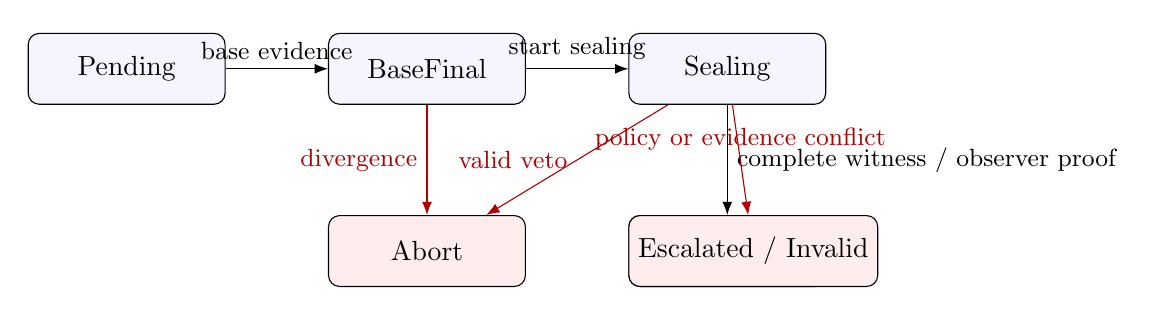
\begin{tikzpicture}[
  >=Latex,
  node distance=1.4cm and 1.3cm,
  state/.style={draw, rounded corners, minimum width=2.5cm, minimum height=0.9cm, align=center, fill=blue!4},
  bad/.style={draw, rounded corners, minimum width=2.5cm, minimum height=0.9cm, align=center, fill=red!7}
]
\node[state] (pending) {Pending};
\node[state, right=of pending] (base) {BaseFinal};
\node[state, right=of base] (sealing) {Sealing};
\node[state, below=of sealing] (sealed) {SealedFinal};
\node[bad, below=of base] (abort) {Abort};
\node[bad, right=of abort] (escalated) {Escalated / Invalid};

\draw[->] (pending) -- node[above, font=\small] {base evidence} (base);
\draw[->] (base) -- node[above, font=\small] {start sealing} (sealing);
\draw[->] (sealing) -- node[right, font=\small] {complete witness / observer proof} (sealed);
\draw[->, red!70!black] (sealing) -- node[left, font=\small] {valid veto} (abort);
\draw[->, red!70!black] (base) -- node[left, font=\small] {divergence} (abort);
\draw[->, red!70!black] (sealing) -- node[above, font=\small] {policy or evidence conflict} (escalated);
\end{tikzpicture}
\caption{The deterministic collapse surface for \code{Asymptote}.}
\end{figure}

\subsection{SealedFinalityProof}

The sealing plane gathers a proof object that binds:

\begin{itemize}[leftmargin=1.5em]
\item the epoch,
\item the achieved finality tier,
\item the collapse state,
\item the guardian manifest hash,
\item the guardian decision hash,
\item the guardian counter,
\item the guardian trace root,
\item the guardian measurement root,
\item the policy hash,
\item witness certificates, when the witness path is used,
\item observer transcripts, transcript commitment, observer challenges,
challenge commitment, and exactly one canonical observer outcome object when
the observer path is used,
\item divergence signals gathered during sealing.
\end{itemize}

This object is block-scoped and guardian-bound. A \code{SealedFinalityProof}
that is not bound to the slot's guardian evidence is invalid.

\subsection{Witness-backed sealing}

The witness path assigns one witness committee per required certification
stratum.

Witness assignment is deterministic over:

\begin{itemize}[leftmargin=1.5em]
\item the epoch seed,
\item the producer account id,
\item the slot \((height, view)\),
\item the reassignment depth,
\item the witness stratum id,
\item the witness manifest hash.
\end{itemize}

Sealed finality is reached on the witness path when:

\begin{itemize}[leftmargin=1.5em]
\item \code{BaseFinal} holds,
\item each required witness stratum contributes a valid assigned witness
certificate,
\item each witness certificate verifies against the registered witness manifest,
\item required checkpoints and append-only proofs are current enough under
policy.
\end{itemize}

Witness omission, stale registry participation, checkpoint inconsistency, or
conflicting witness certificates produce explicit evidence rather than silent
best-effort behavior.

\subsection{Equal-authority observer sealing}

The normative observer path is \code{CanonicalChallengeV1}. It treats sampled
validators as deterministic duty assignees whose outputs must become public,
recoverable protocol objects.

Observer assignment is deterministic over:

\begin{itemize}[leftmargin=1.5em]
\item the epoch seed,
\item the producer account id,
\item the slot \((height, view)\),
\item the observation round,
\item the observer account id.
\end{itemize}

The producer is excluded from its own observer pool. The runtime may also
filter assignments through a correlation budget over provider, region, host
class, and key-authority class.

Each assigned observer publishes one of two things:

\begin{itemize}[leftmargin=1.5em]
\item a guardian-backed \code{AsymptoteObserverTranscript}, or
\item an objective \code{AsymptoteObserverChallenge}.
\end{itemize}

A transcript binds the canonical slot surface:

\begin{itemize}[leftmargin=1.5em]
\item the epoch and assignment,
\item the candidate block hash,
\item the guardian manifest, decision hash, counter, trace hash, and
measurement root,
\item the guardian checkpoint root,
\item the observer verdict and veto kind,
\item the observer evidence hash.
\end{itemize}

The admissible challenge basis is public-evidence-only:

\begin{itemize}[leftmargin=1.5em]
\item \code{MissingTranscript},
\item \code{TranscriptMismatch},
\item \code{VetoTranscriptPresent},
\item \code{ConflictingTranscript},
\item \code{InvalidCanonicalClose}.
\end{itemize}

Each challenge carries its own public evidence object: an assignment, an
offending observation request, an offending transcript, or an offending
canonical close. The challenge \code{evidence\_hash} must bind exactly that
carried evidence.

The slot then carries three canonical bindings:

\begin{itemize}[leftmargin=1.5em]
\item a transcript commitment over the transcript surface,
\item a challenge commitment over the challenge surface,
\item exactly one canonical outcome object:
  \code{AsymptoteObserverCanonicalClose} or
  \code{AsymptoteObserverCanonicalAbort}.
\end{itemize}

The collapse rule is close-or-abort and challenge-dominant:

\begin{itemize}[leftmargin=1.5em]
\item \code{SealedFinal} if \code{BaseFinal} holds, the deterministic
assignment set is fully covered by valid canonical \code{Ok} transcripts, the
transcript and challenge commitments verify, the challenge surface is empty,
and the canonical close object is valid.
\item \code{Abort} if the transcript and challenge commitments verify, the
challenge surface is non-empty, and the canonical abort object is valid.
\item \code{Pending} otherwise.
\end{itemize}

Challenge dominance is a theorem-level veto, not an operational alarm. A valid
challenge collapses the slot to abort before any penalty, governance, or
membership aftermath is considered.

This makes observer sealing structurally parallel to canonical ordering:
public evidence, canonical commitments, a unique positive object, a unique
negative object, and deterministic local close-or-abort derivation from the
same public surface.

\subsection{Divergence signals and escalation}

The sealing plane may also emit divergence signals, including:

\begin{itemize}[leftmargin=1.5em]
\item conflicting guardian certificates,
\item witness omission,
\item stale registry use,
\item stale checkpoints,
\item transparency-log consistency failure.
\end{itemize}

These signals support \code{Escalated} and \code{Invalid} outcomes and give
operators a fail-closed evidence trail.

\subsection{Sealed effects and replay-safe release}

Irreversible effects are gated by finality tier. The effect plane
distinguishes between:

\begin{itemize}[leftmargin=1.5em]
\item \code{BaseFinal} effects, which are allowed on the fast path when policy
permits,
\item \code{SealedFinal} effects, which require a valid
\code{SealedFinalityProof}.
\end{itemize}

For proof-enabled irreversible effects, \code{Asymptote} carries a
self-contained \code{SealObject} whose current instantiation includes:

\begin{itemize}[leftmargin=1.5em]
\item an \code{EffectIntent},
\item an \code{EffectPublicInputs} object, including
  \code{canonical\_collapse\_hash},
\item an \code{EffectProofEnvelope},
\item a replay-safe nullifier.
\end{itemize}

In the runtime, \code{SealedFinal} secure-egress requests carry both
the \code{SealedFinalityProof} and the slot's
\code{CanonicalCollapseObject}. The guardian-side seal builder and downstream
receipt verifier recompute the same \code{canonical\_collapse\_hash} from that
collapse object together with the proof-carried observer surface, so a
challenge-dominated or otherwise mismatched slot cannot authorize irreversible
release.

The release rule is
\[
\mathrm{Release}(e)
\iff
\mathrm{BaseFinal}(\mathrm{slot}(e))
\wedge
\mathrm{SealedFinal}(\mathrm{slot}(e))
\wedge
\mathrm{VerifySealObject}(e)
\wedge
\mathrm{CollapseHash}(e)=\mathrm{Hash}(\mathrm{Collapse}(\partial_h))
\wedge
\neg \mathrm{NullifierUsed}(e).
\]

This keeps the hot path sparse while making released consequences deterministic
and replay-safe.

\subsection{Deterministic observer theorem}

The deterministic \code{Asymptote} observer model now proves the following
kernel:

\begin{itemize}[leftmargin=1.5em]
\item base certificates are unique per slot,
\item canonical observer close objects are unique per slot,
\item canonical observer close and canonical observer abort cannot coexist for
the same slot,
\item a challenge-dominated slot cannot produce a valid sealed release.
\end{itemize}

\begin{theorem}[Deterministic Equal-Authority Observer Sealing]
Assume sound deterministic observer assignment, signature-sound guardian-backed
observer transcripts and challenges, canonical transcript and challenge
commitments, append-only registry and log publication once published, and
deterministic transcript/challenge derivation over the closed public observer
surface. Then arbitrary behavior by the rest of the validator set cannot create a
conflicting valid canonical observer close, cannot make canonical close and
canonical abort coexist for the same slot, and cannot authorize a valid sealed
irreversible effect release for a challenge-dominated slot.
\end{theorem}

This theorem is the observer-lane analogue of canonical ordering's public
certificate theorem: public evidence, canonical commitments, negative-authority
dominance, and deterministic local close-or-abort derivation from the same
public observer surface.

Under the accountable publication rules of
Section~\ref{sec:system-model}, the same observer challenges are also
penalty-bearing objective faults. Unsafe positive close attempts therefore
become not only rejectable, but accountable and epoch-removing.

\subsection{Legacy sampled comparison}

Before \code{CanonicalChallengeV1}, the observer lane was typically described
through a sampled affirmative bound. Let:

\begin{itemize}[leftmargin=1.5em]
\item \(h\) be the honest fraction of equal-authority validators,
\item \(A_s^j\) be the sampled observer committee for slot \(s\) and round
\(j\),
\item \(k_j = |A_s^j|\),
\item \(p_{\mathrm{beacon\_bias}}\) be the probability of sufficient beacon
bias,
\item \(p_{\mathrm{veto\_suppression}}\) be the probability that a valid veto
surface is fully suppressed.
\end{itemize}

Then the old affirmative sampled lane admitted the analytical bound
\[
P_{\mathrm{unsafe}}(s)
\le
p_{\mathrm{beacon\_bias}}
\cdot
p_{\mathrm{veto\_suppression}}
\cdot
\prod_j (1 - h)^{k_j}.
\]

For constant committee size \(k\) across \(r\) rounds:
\[
P_{\mathrm{unsafe}}(s)
\le
p_{\mathrm{beacon\_bias}}
\cdot
p_{\mathrm{veto\_suppression}}
\cdot
(1 - h)^{kr}.
\]

That formula remains a useful historical comparison, but it is no longer the
normative theorem for the observer lane. Under \code{CanonicalChallengeV1},
sampling determines duties, not safety. Safety comes from the canonical public
transcript surface, the canonical public challenge surface, and the
close-or-abort split that those surfaces induce.

The runtime publishes the canonical observer transcript, commitment, challenge,
challenge commitment, and close-or-abort objects as ordinary
\code{guardian\_registry} transactions after the sealed header is formed. The
same surface is carried inside the proof for immediate block verification.

\section{NestedGuardian: Witness-Augmented Research Mode}

\code{NestedGuardian} explores a layered threshold construction:

\begin{itemize}[leftmargin=1.5em]
\item validators run the \AFT{} deterministic message flow,
\item each proposal carries its guardian committee certificate,
\item external witness committees cross-check the slot,
\item chain state anchors witness assignments, witness manifests, and slashing
evidence.
\end{itemize}

The instantiated runtime scope includes:

\begin{itemize}[leftmargin=1.5em]
\item deterministic witness assignment from the active witness set,
\item registered on-chain witness manifests,
\item witness certificates bound into guardianized slot certificates,
\item safety proofs for the witness-augmented kernel,
\item bounded model checking for reassignment, outage, and checkpoint
transitions.
\end{itemize}

The instantiated proof package consists of:

\begin{itemize}[leftmargin=1.5em]
\item safety formalization,
\item bounded operational model checking for reassignment, outage, and
checkpoint transitions,
\item a discharged composed-liveness bridge under the target eventual-fair
scheduler through the recurrence/reduction/totality/collapse chain together
with a matching persistent churn/restart simulator.
\end{itemize}

\code{NestedGuardian} is therefore a witness-augmented mode with a finished
theorem bridge. It is experimental as an operational mode, not as a theorem
crutch. Its witness-coded family supplies an explicit constructive recovery
carrier and completed bridge artifacts; it does not reduce the promoted
\AFT{} theorem surface to an experimental-only claim. That constructive
recovery carrier is a witness-coded publication-bundle recovery contract with
compact hot-path bindings and cold-path registry-driven close-or-abort
resolution. The abstract coded
recovery-family contract is realized by the parametric
\code{SystematicXorKOfKPlus1V1} parity family plus the bounded true non-parity
\code{SystematicGf256KOfNV1} family with at least two parity shares,
implemented with systematic Cauchy-style coefficients and exercised in bounded
\code{2-of-4}, \code{3-of-5}, \code{3-of-7}, \code{4-of-6}, and \code{4-of-7}
lanes. These lanes resolve from threshold-many public reveals, objective
recovered-support conflict, or deterministic missingness. The bounded
\code{3-of-5}, \code{4-of-6}, and \code{4-of-7} lanes restore or exceed
threshold-support overlap while the bounded \code{3-of-7} lane shows that
recovered-support conflict remains fail-closed even when overlap is absent. A
bounded conformance harness checks that every threshold-sized reveal subset
reconstructs and every below-threshold subset fails across the shipped XOR and
GF256 realizations of that contract. Those recovered reveals lift
deterministically into an explicit positive close-extraction payload and then
into an explicit extractable bulletin-surface payload that binds the verifying
publication bundle, verifying canonical bulletin close, canonical
bulletin-availability bytes, and sorted bulletin entries.

The completed bounded family also carries the ordinary durable and restart
surfaces. A bounded recovered-only two-slot harness shows that consecutive
recovered surfaces derive the ordinary publication-frontier predecessor chain
and the same authoritative \code{CanonicalCollapseObject} predecessor chain
without the ordinary publication-bundle lane. A second bounded recovered-only
harness shows a close/abort/close bulletin window with a recovered
omission-dominated middle slot: recovered data alone materializes the ordinary
positive closes and extracted bulletin surfaces on the outer slots,
materializes the ordinary omission-dominated abort in the middle while keeping
omission evidence and recovered bulletin entries public, and preserves the same
authoritative collapse continuity chain. A bounded read-side harness shows that
the same recovered-only durable chain yields the same compact replay-prefix /
state-root continuity view that the ordinary lane exposes plus a bounded
recovered canonical-header prefix. The execution module verifies that replay
tip as the same restart anchor the ordinary lane uses, retains both recovered
prefixes in execution state, and uses the recovered canonical-header ancestry
for bounded anchored reads plus parent-block / parent-state-root continuity
after restart when ordinary recent blocks are absent.

Validator consensus orchestration derives the same bounded recovered restart
parent anchor from the recovered canonical-header / collapse surface when the
ordinary committed block is absent, and the \code{GuardianMajority} engine
consumes that bounded recovered canonical-header prefix as restart-time
parent/QC context for synthetic parent-height QC continuity when the full
committed block is absent. The same recovered surface yields a bounded
recovered certified-header window plus a restart-only recovered
\code{BlockHeader} / QC cache window for restart-time header / QC lookup plus
bounded QC-certified recovered branch reconciliation over the configured local
five-entry window. Those windows fold by exact overlap with a configurable
budget, exercised at five windows into a longer seventeen-step recovered
certified branch without ordinary committed headers. Those same cold-path
loaders consume a configurable exact-overlap segment budget, exercised at four
exact-overlap segments into a longer fifty-three-step recovered certified
branch with direct registry-extraction parity and explicit interior-overlap
conflict rejection. Those same restart loaders also compose two overlapping
four-segment exact-overlap folds into a longer eighty-nine-step recovered
certified branch with direct registry-extraction parity and explicit inter-fold
overlap conflict rejection, and tests exercise the same recursive carrier at
three overlapping four-segment folds into a one-hundred-twenty-five-step
recovered certified branch. The runtime has a bounded conformance harness over
one, two, and three stitched segment folds, matching the same production-loader
/ registry-extraction carrier at the corresponding fifty-three-step,
eighty-nine-step, and one-hundred-twenty-five-step branches.

The restart path also pages older exact-overlap segment folds on demand beneath
that bounded suffix via an overlap-checked cursor while keeping only the
bounded recent suffix plus the streamed page live in engine caches, and tests
exercise that paged carrier at a longer two-hundred-thirty-three-step
recovered certified branch with direct registry-extraction parity plus explicit
duplicate-page, missing-gap, and late-page overlap rejection. Restart
therefore streams recovered certified ancestry until target height or
recovered-history exhaustion without a theorem-relevant fixed depth bound.

The archival internalization layer uses an active archived-recovered-history
profile naming retention horizon, exact-overlap paging geometry, segment /
fold geometry, checkpoint update rule, and profile evolution. Archived
segments, archived restart pages, archival checkpoints, and archival retention
receipts bind to historically referenced profile hashes and governing
activation hashes under a published profile-activation chain before archived
continuation is trusted, and ordinary canonical collapse history names the
archived checkpoint / activation pair that archived restart is authorized to
follow. Archived replay and archived publication correctness are historical and
index-free: they follow the canonical-collapse-anchored or object-carried
activation hash plus predecessor/checkpoint history rather than whichever
archived activation is merely latest in local state.

When the recovered certificate carries objective omission proofs, the same
recovered lane routes into the ordinary \code{OmissionDominated} abort path
while keeping omission evidence and recovered bulletin entries public. The
recovery-family contract, canonical-collapse / replay retrievability anchor, and
recovered-state historical retrievability surface are therefore part of ordinary endogenous
\AFT{} history rather than a narrower theorem-side qualifier. The directly
discharged recurrence/reduction/totality/collapse chain closes the former
distance to unconditional classical \code{99\% Byzantine agreement}, so no
lower-bound, recoverability, or architecture-specific semantic gap remains at
the theorem surface.

\section{Security and Assumption Surface}

The \AFT{} family depends on explicit assumptions. They are not optional prose.

\begin{center}
\small
\begin{tabularx}{\textwidth}{>{\raggedright\arraybackslash}p{0.17\textwidth} >{\raggedright\arraybackslash}p{0.42\textwidth} X}
\toprule
\textbf{Layer} & \textbf{Required assumptions} & \textbf{Failure consequence} \\
\midrule
Base finality & current manifests, current epoch state, majority thresholds, guardian non-equivocation, valid checkpoints, enough validators and guardians to reach quorum & conflicting base-finality evidence or loss of progress \\
Canonical ordering & objective publication, compact publication-frontier binding and contradiction rules, canonical cutoff, deterministic eligibility, append-only bulletin commitment, proof soundness, protocol-native retrievability profile / manifest / custody / challenge surface, canonical bulletin-close extraction-or-abort, cheap omission verification, accountable omission publication & loss of compact frontier consistency, deterministic extraction-or-abort, accountability, or the ordering theorem \\
Sealed finality & valid asymptote policy, current witness seed, valid witness or observer assignments, checkpoint freshness, valid log consistency proofs, deterministic transcript/challenge derivation, accountable challenge publication & incorrect sealed release, loss of accountability, or fail-closed stalling \\
Sealed effects & correct finality-tier policy, sound verifier metadata, nullifier uniqueness, intent/public-input binding & replay or unsafe irreversible effect release \\
NestedGuardian & sound witness assignment and registration, correct reassignment handling, witness committee non-equivocation & degraded safety or open liveness behavior \\
\bottomrule
\end{tabularx}
\end{center}

The family-level discipline is simple: if an assumption fails, \AFT{} should
degrade to stalling, aborting, or withholding release before it degrades to
unsafe irreversible behavior.

\section{Formal Results}

The repository's machine-checked surfaces align with the protocol family as
follows:

\begin{center}
\scriptsize
\begin{tabularx}{\textwidth}{>{\raggedright\arraybackslash}p{0.28\textwidth} X}
\toprule
\textbf{Formal module} & \textbf{Core proved results} \\
\midrule
\code{GuardianMajorityProof} & \code{QuorumCertificatesIntersect}, \code{InvariantImpliesSafety} \\
\code{GuardianMajority} & executable bounded checks for finalization witness soundness and slot safety \\
\code{CanonicalOrderingProof} & \shortstack[l]{\code{InvariantImpliesCertifiedUniqueness},\\\code{InvariantImpliesRecoverability},\\\code{InvariantImpliesOmissionDominates}} \\
\code{CanonicalOrdering} & executable bounded checks for publication, cutoff, certification, omission, and recoverability \\
\code{AsymptoteProof} & \shortstack[l]{\code{InvariantImpliesBaseSafety},\\\code{InvariantImpliesCanonicalCloseSafety},\\\code{InvariantImpliesCloseAbortExclusive},\\\code{InvariantImpliesAbortDominatesSealed}} \\
\code{Asymptote} & executable bounded checks for transcript publication, challenge publication, canonical close, and canonical abort \\
\code{NestedGuardianProof} & \shortstack[l]{witness-assignment soundness,\\witness-certificates-stay-assigned,\\\code{InvariantImpliesSafety}} \\
\code{NestedGuardian} & executable bounded checks for reassignment, outage, and checkpoint admissibility \\
\bottomrule
\end{tabularx}
\end{center}

Every formal artifact named in this section, and every additional proof
artifact cited by file name below, is embedded verbatim in
Appendix~\ref{appendix:formal-artifacts} so that the served yellow paper
remains self-contained outside the repository.

These formal surfaces prove the deterministic safety kernels that the broader
classical-agreement bridge builds on. The full ordinary classical
\code{99\% Byzantine agreement} sentence is then completed by the recurring,
reduction, totality, and collapse layers discussed above, rather than by these
module-local safety kernels in isolation. Compact publication-frontier
summaries internalize same-slot and predecessor consistency on the live path,
while the protocol-native retrievability plane internalizes closed-bulletin
extraction-or-abort as an endogenous part of the realizing architecture rather
than a purely algebraic consequence of the authenticated message transcript
alone.

The accountable-adversary variant therefore composes these formal kernels with
runtime accountability rules rather than replacing them: replay-deduplicated
objective fault publication and optional policy-controlled membership updates
live in the implementation and policy layer above the proved
deterministic core.

\subsection{Complete omission-dominance witness artifact}

The formal package includes an executable TLC witness module,
\code{docs/architecture/consensus/aft/formal/canonical\_ordering/CanonicalOrderingOmissionTrace.tla},
paired with
\code{docs/architecture/consensus/aft/formal/canonical\_ordering/CanonicalOrderingOmissionTrace.cfg}.
The exact module and configuration are embedded in
Appendix~\ref{app:co-omission-trace} and
Appendix~\ref{app:co-omission-trace-cfg}; the summary below highlights the
executed public-evidence shape that the witness reaches.

\paragraph{Executed witness trace.}
The module intentionally asks TLC to violate the state predicate
\code{NoOmissionDominanceWitness} so that the checker emits a concrete public
evidence trace. The executed trace is:

\begin{enumerate}[leftmargin=1.5em]
\item \code{PublishStep}: \code{tx1} enters slot \(1\)'s bulletin surface.
\item \code{PublishStep}: \code{tx2} enters the same bulletin surface.
\item \code{CloseCutoffStep}: the canonical cutoff closes and the recoverable
set becomes \(\{tx1, tx2\}\).
\item \code{CandidateCertifyStep}: a candidate certificate for \(\{tx1\}\)
appears.
\item \code{ProveOmissionStep}: an omission proof for \(tx2\) against that
candidate certificate appears.
\end{enumerate}

The same formal package carries a bounded recursive-continuity model,
\code{docs/architecture/consensus/aft/formal/canonical\_ordering/CanonicalCollapseRecursiveContinuity.tla},
paired with
\code{docs/architecture/consensus/aft/formal/canonical\_ordering/CanonicalCollapseRecursiveContinuity.cfg}.
The exact source of both artifacts is embedded in
Appendix~\ref{app:co-recursive-continuity} and
Appendix~\ref{app:co-recursive-continuity-cfg}.
That model captures the reference \code{HashPcdV1} continuity carrier directly:
deterministic recursive proof steps, predecessor-proof hashing,
\code{CanonicalCollapseExtensionCertificate} carriage, and the rule that
non-genesis header admission depends on the anchored predecessor proof relation.
The runtime exposes a \code{SuccinctSp1V1} backend seam for those
same recursive public inputs, and that seam is exercised by consensus
verification and durable-state gating. The formal model still stops at the
reference carrier rather than mechanizing a cryptographic recursive
accumulator or ZK backend.

At the final state, the incomplete candidate certificate remains
\emph{unadmitted} while the omission proof is present. In the executable
model this happens because the admitted object must already equal the canonical
set; the trace therefore does not replace the theorem. Its purpose is narrower
and useful: it gives a bounded, executed witness of the exact public-evidence
shape from which omission dominance follows. Readers can run the trace directly
and inspect the six-state witness without reconstructing the paper's argument by
hand.

\section{Implementation Correspondence}

This section is non-normative. It names the exact runtime symbols that carry
the protocol objects defined above.

\subsection{Core ordering symbols}

The core ordering data structures and free functions are public Rust symbols
re-exported through \code{ioi\_types::app}. They are the runtime carriers for
the abstract ordering objects and verifier rules defined above.

\begin{center}
\scriptsize
\begin{tabularx}{\textwidth}{>{\raggedright\arraybackslash}p{0.32\textwidth} X}
\toprule
\textbf{Abstract object} & \textbf{Current runtime symbols} \\
\midrule
Bulletin surface commitment & \code{BulletinCommitment}, \code{BulletinSurfaceEntry} \\
Compact publication availability binding & \code{PublicationAvailabilityReceipt} \\
Compact publication frontier & \code{PublicationFrontier} \\
Publication-frontier contradiction & \code{PublicationFrontierContradiction} \\
Canonical ordering proof families & \code{CanonicalOrderProofSystem}, with concrete variants \code{HashBindingV1} and \code{CommittedSurfaceV1} \\
Canonical public-input tuple & \code{CanonicalOrderPublicInputs} \\
Live succinct witness payload & \code{CommittedSurfaceCanonicalOrderProof} \\
Omission evidence & \code{OmissionProof} \\
Order certificate & \code{CanonicalOrderCertificate} \\
Canonical ordering function & \code{canonical\_order\_tx\_hashes} \\
Publication-frontier hashing & \shortstack[l]{\code{canonical\_publication\_availability}\\\code{\_receipt\_hash},\\\code{canonical\_publication\_frontier\_hash},\\\code{canonical\_publication\_frontier}\\\code{\_contradiction\_hash}} \\
Publication-frontier construction / verification & \shortstack[l]{\code{build\_publication\_availability\_receipt},\\\code{build\_publication\_frontier},\\\code{verify\_publication\_frontier},\\\code{verify\_publication\_frontier\_contradiction}} \\
Public-input hashing & \shortstack[l]{\code{canonical\_order\_public\_inputs},\\\code{canonical\_order\_public\_inputs\_hash}} \\
Reference proof construction & \shortstack[l]{\code{build\_reference\_canonical\_order}\\\code{\_proof\_bytes}} \\
Live certificate construction & \shortstack[l]{\code{build\_committed\_surface\_canonical}\\\code{\_order\_certificate}} \\
Certificate verification & \code{verify\_canonical\_order\_certificate} \\
\bottomrule
\end{tabularx}
\end{center}

\subsection{Guardian and sealing symbols}

The guardian, witness, observer, and sealed-effect objects are likewise public
Rust symbols re-exported through \code{ioi\_types::app}. They encode the exact
evidence surface checked by validators and downstream gateways.

\begin{center}
\small
\begin{tabularx}{\textwidth}{>{\raggedright\arraybackslash}p{0.32\textwidth} X}
\toprule
\textbf{Abstract object} & \textbf{Current runtime symbols} \\
\midrule
Guardian slot certificate & \code{GuardianQuorumCertificate} \\
Witness certificate & \code{GuardianWitnessCertificate} \\
Equal-authority observer assignment & \code{AsymptoteObserverAssignment} \\
Correlation budget & \code{AsymptoteObserverCorrelationBudget} \\
Observer observation request & \code{AsymptoteObserverObservationRequest} \\
Observer transcript & \code{AsymptoteObserverTranscript} \\
Observer transcript commitment & \code{AsymptoteObserverTranscriptCommitment} \\
Observer challenge & \code{AsymptoteObserverChallenge}, with kinds \code{MissingTranscript}, \code{TranscriptMismatch}, \code{VetoTranscriptPresent}, \code{ConflictingTranscript}, and \code{InvalidCanonicalClose} \\
Observer challenge commitment & \code{AsymptoteObserverChallengeCommitment} \\
Canonical observer close & \code{AsymptoteObserverCanonicalClose} \\
Canonical observer abort & \code{AsymptoteObserverCanonicalAbort} \\
Finality tier & \code{FinalityTier}, with variants \code{BaseFinal} and \code{SealedFinal} \\
Collapse state & \code{CollapseState}, with variants \code{Pending}, \code{BaseFinal}, \code{Sealing}, \code{Abort}, \code{SealedFinal}, \code{Escalated}, and \code{Invalid} \\
Sealing policy & \code{AsymptotePolicy} \\
Observer statement & \code{AsymptoteObserverStatement} \\
Observer certificate & \code{AsymptoteObserverCertificate} \\
Divergence signal & \code{DivergenceSignal}, \code{DivergenceSignalKind} \\
Sealed finality proof & \code{SealedFinalityProof} \\
Observer binding for sealed effects & \code{sealed\_finality\_proof\_observer\_binding} \\
Proof-carrying effect object & \code{SealObject} \\
\bottomrule
\end{tabularx}
\end{center}

\subsection{Verifier, orchestration, and persistence symbols}

Verification and orchestration entry points are split across four public
namespaces: \code{ioi\_types::app},
\code{ioi\_crypto::sign::guardian\_committee},
\code{ioi\_services::guardian\_registry}, and the
\code{GuardianMajorityEngine} runtime. Engine-local checks are named here by
their exact method identifiers.

\begin{center}
\scriptsize
\begin{tabularx}{\textwidth}{>{\raggedright\arraybackslash}p{0.37\textwidth} X}
\toprule
\textbf{Responsibility} & \textbf{Current runtime symbols} \\
\midrule
Guardian certificate verification & \code{verify\_quorum\_certificate} \\
Witness certificate verification & \code{verify\_witness\_certificate} \\
Deterministic observer assignment & \shortstack[l]{\code{derive\_asymptote\_observer\_assignments},\\\code{derive\_asymptote\_observer\_plan\_entries}} \\
Observer-side transcript / challenge derivation & \shortstack[l]{\code{GuardianContainer::observe\_asymptote\_request},\\\code{GuardianContainer::request\_remote\_asymptote}\\\code{\_observer\_observation},\\\code{GuardianContainer::sign\_consensus\_with\_guardian}} \\
Sealed finality verification in the engine & \shortstack[l]{\code{GuardianMajorityEngine::verify\_asymptote}\\\code{\_canonical\_observer\_sealed\_finality},\\\code{GuardianMajorityEngine::verify\_asymptote}\\\code{\_sealed\_finality}} \\
Canonical-order enrichment verification in the engine & \shortstack[l]{\code{GuardianMajorityEngine::verify}\\\code{\_canonical\_order\_enrichment}; published\\\code{CanonicalOrderAbort} dominates positive order\\certificates and inconsistent mixed parent state} \\
Publication-frontier enrichment verification in the engine & \shortstack[l]{\code{GuardianMajorityEngine::verify}\\\code{\_publication\_frontier\_enrichment}; published\\\code{PublicationFrontierContradiction} dominates\\conflicting or stale frontiers} \\
Block finalization attachment of order certificates & \shortstack[l]{\code{build\_committed\_surface\_canonical}\\\code{\_order\_certificate} during finalization} \\
Block finalization attachment of publication frontier & \code{build\_publication\_frontier} during finalization \\
Canonical observer proof publication & \shortstack[l]{\code{canonicalize\_observer\_sealed\_finality\_proof},\\\code{publish\_canonical\_observer\_artifacts}} \\
Sealed-effect construction and checking & \code{build\_http\_egress\_seal\_object}, \code{verify\_seal\_object} \\
Guardianized proposal verification in the engine & \shortstack[l]{\code{GuardianMajorityEngine::verify}\\\code{\_guardianized\_certificate}} \\
Base-engine safety and timing & \code{SafetyGadget}, \code{Pacemaker}, \code{TimeoutCertificate} \\
Bulletin and order-certificate state access & \shortstack[l]{\code{load\_bulletin\_commitment},\\\code{load\_canonical\_order\_certificate}} \\
Publication-frontier state access & \shortstack[l]{\code{GuardianRegistry::load\_publication\_frontier},\\\code{GuardianRegistry::load\_publication}\\\code{\_frontier\_contradiction}} \\
Ordering close-or-abort derivation & \shortstack[l]{\code{derive\_canonical\_order\_execution\_object},\\\code{derive\_canonical\_order\_public\_obstruction}} \\
Ordering abort taxonomy & \shortstack[l]{\code{CanonicalOrderAbortReason::MissingOrderCertificate},\\\code{BulletinSurfaceReconstructionFailure},\\\code{BulletinSurfaceMismatch},\\\code{InvalidBulletinClose},\\\code{OmissionDominated},\\\code{CertificateHeightMismatch},\\\code{RandomnessMismatch},\\\code{OrderedTransactionsRootMismatch},\\\code{ResultingStateRootMismatch},\\\code{InvalidPublicInputsHash},\\\code{InvalidBulletinAvailabilityCertificate},\\\code{InvalidProofBinding}} \\
Protocol-wide collapse derivation and verification & \shortstack[l]{\code{derive\_canonical\_collapse\_object},\\\code{GuardianMajorityEngine::verify\_published}\\\code{\_canonical\_collapse\_object}} \\
Proposal-surface recursive continuity & \shortstack[l]{\code{BlockHeader::previous\_canonical\_collapse\_commitment\_hash},\\\code{BlockHeader::canonical\_collapse\_extension\_certificate},\\\code{CanonicalCollapseExtensionCertificate},\\\code{CanonicalCollapseCommitment},\\\code{verify\_block\_header\_canonical\_collapse\_evidence},\\\code{ConsensusDecision::ProduceBlock}} \\
Bulletin, order, and collapse state access & \shortstack[l]{\code{load\_bulletin\_commitment},\\\code{load\_canonical\_order\_certificate},\\\code{load\_canonical\_order\_abort},\\\code{load\_canonical\_collapse\_object}} \\
On-chain publication verbs & \shortstack[l]{\code{publish\_aft\_publication\_frontier@v1},\\\code{publish\_aft\_canonical\_order\_artifact\_bundle@v1},\\\code{publish\_aft\_canonical\_order\_abort@v1},\\\code{publish\_aft\_canonical\_collapse\_object@v1},\\\code{report\_aft\_omission@v1},\\\code{publish\_asymptote\_observer\_transcript@v1},\\\code{publish\_asymptote\_observer\_transcript\_commitment@v1},\\\code{report\_asymptote\_observer\_challenge@v1},\\\code{publish\_asymptote\_observer\_challenge\_commitment@v1},\\\code{publish\_asymptote\_observer\_canonical\_close@v1},\\\code{publish\_asymptote\_observer\_canonical\_abort@v1}} \\
Accountable evidence replay protection and validator removal & \shortstack[l]{\code{evidence\_id},\\\code{GuardianRegistry::apply\_accountable\_fault\_report},\\\code{GuardianRegistry::apply\_accountable\_membership\_updates}} \\
Native benchmark target & \code{benchmark\_throughput} \\
\bottomrule
\end{tabularx}
\end{center}

These symbols are named here so that the paper maps directly onto the current
runtime without making the reader chase separate prose specifications. In the
implementation, validator finalization publishes a protocol-visible
\code{CanonicalCollapseObject} through
\code{publish\_aft\_canonical\_collapse\_object@v1} after local post-commit
header enrichment, \code{guardian\_registry} exposes
\code{load\_canonical\_collapse\_object}, and
\code{GuardianMajorityEngine::verify\_published\_canonical\_collapse\_object}
cross-checks any published copy against the proof-carried header surface when
it is available. The externally finalized AFT commit path persists the same
object keyed by slot height, rather than treating ordering and sealing
close-or-abort evidence as loose enrichments detached from state persistence.
The same post-commit path also builds \code{PublicationFrontier} via
\code{build\_publication\_frontier} and publishes it through
\code{publish\_aft\_publication\_frontier@v1};
\code{GuardianMajorityEngine::verify\_publication\_frontier\_enrichment}
rechecks same-slot binding, predecessor linkage, and any dominating
contradiction object.
In the current proposal-surface continuity slice, validator orchestration now
signs both \code{previous\_canonical\_collapse\_commitment\_hash} and a typed
\code{CanonicalCollapseExtensionCertificate} into each produced AFT block
header.
In the current clean-break runtime slice, \code{CanonicalCollapseObject}
itself carries \code{continuity\_accumulator\_hash} and
\code{continuity\_recursive\_proof}, so the certificate now carries the
predecessor commitment plus predecessor proof hash rather than an explicit
carried ancestor vector, full predecessor collapse object, or predecessor
recursive proof object.
\code{Asymptote} leaders stall rather than produce when that required
extension certificate is unavailable, proposal verification recursively
checks that the carried predecessor commitment hash matches the signed
predecessor link, checks that the predecessor commitment's resulting state root matches the
signed parent-state root, and rechecks those carried public inputs against the
anchored predecessor collapse object when one is available. QC promotion
therefore relies on a reference recursive proof-carrying continuity relation
rather than on a recomputed predecessor digest alone, and only treats continuity-linked
headers as progress-bearing.

\section{Benchmark Context}

The performance evidence in this paper has two sources:

\begin{itemize}[leftmargin=1.5em]
\item literature-reported baselines for \code{HotStuff}, \code{Narwhal/Tusk},
and \code{Bullshark},
\item the repository's native \code{benchmark\_throughput} target for matched
\code{GuardianMajority} and \code{Asymptote} scenarios.
\end{itemize}

The purpose of this section is architectural positioning, not false
equivalence across unmatched environments.

\subsection{Paper-reported baselines}

\begin{center}
\small
\begin{tabularx}{\textwidth}{>{\raggedright\arraybackslash}p{0.28\textwidth} >{\raggedleft\arraybackslash}p{0.16\textwidth} >{\raggedleft\arraybackslash}p{0.16\textwidth} X}
\toprule
\textbf{System} & \textbf{Reported throughput} & \textbf{Reported latency} & \textbf{Source type} \\
\midrule
HotStuff baseline & 1{,}800 tx/s & 1 s & Narwhal/Tusk comparison setting \\
Narwhal-HotStuff & 130{,}000 tx/s & under 2 s & Narwhal/Tusk paper \\
Narwhal-HotStuff with additional workers & up to 600{,}000 tx/s & n/a & Narwhal/Tusk paper \\
Tusk & 160{,}000 tx/s & about 3 s & Narwhal/Tusk paper \\
Bullshark & 125{,}000 tx/s & about 2 s & Bullshark paper \\
\bottomrule
\end{tabularx}
\end{center}

The baseline interpretation is:

\begin{itemize}[leftmargin=1.5em]
\item \code{HotStuff} demonstrates the leader-based partially synchronous
baseline,
\item \code{Narwhal-HotStuff} demonstrates the gain from separating
dissemination from ordering,
\item \code{Bullshark} demonstrates high-throughput DAG-oriented ordering,
\item \AFT{} adds a new separation: order surfacing and effect release are no
longer identified with dense positive voting.
\end{itemize}

\subsection{Native repository measurements}

No performance measurement in this section is load-bearing for any theorem in
this paper; the promoted theorem surface stands independently of benchmark
tuning, harness state, or optimization maturity.

The corrected native measurements below were produced on March 21, 2026 after
bringing the repository's native AFT benchmark path back into sync with the
current \code{GuardianMajority} / \code{base\_final} harness semantics:

\begin{itemize}[leftmargin=1.5em]
\item shared-tip readiness no longer treats a transient
\code{get\_status.height = 0} as authoritative when a resilient tip probe
already sees committed blocks,
\item submission alignment and leader-targeted ingress now use a resilient tip
block rather than a potentially stale status height,
\item authoritative chain-commit scans start from the resilient
pre-submission tip instead of rescanning stale empty-block prefixes,
\item sustained throughput for fast probes now stops on the authoritative
full-chain commit scan for the highest committed height; sampled committed-status
visibility is retained only as an auxiliary lag diagnostic,
\item the benchmark surface now exposes alignment, spill, and replay
diagnostics explicitly so missed due blocks or replay churn are not hidden
behind a single TPS number.
\end{itemize}

The table below reports the current matched bulk-throughput proof point for the
native \code{GuardianMajority} 4-validator \code{base\_final} scenario under
that corrected harness. This is a repository-native AFT proof point on the
Jellyfish state path with a `1 s` block interval, not an apples-to-apples claim
against published Narwhal/Tusk/Bullshark environments.

\begin{center}
\scriptsize
\resizebox{\textwidth}{!}{%
\begin{tabular}{lrrrrrrrrrrrr}
\toprule
scenario & validators & attempted & accepted & committed & blocks & inj. tps & sust. tps & p50 & p95 & p99 & sealed p50 & sealed p95 \\
\midrule
guardian\_majority\_4v\_base\_final\_bulk & 4 & 16384 & 16384 & 16384 & 1 & 21370.89 & 9647.66 & 1293.45 & 1603.73 & 1695.24 & -- & -- \\
\bottomrule
\end{tabular}%
}
\end{center}

These measurements imply four things:

\begin{itemize}[leftmargin=1.5em]
\item the earlier single-digit and low-hundreds TPS reports were artifacts of
benchmark-path bugs rather than of the protocol surface itself,
\item the current repository now clears the lower edge of the intended
\code{8k--16k TPS} range in a matched native 4-validator
\code{GuardianMajority} bulk probe,
\item on this corrected probe the batch lands in a single block, so the main
remaining AFT work is ceiling-raising and aggregate-domain multiplication rather
than recovering from a broken harness,
\item these values should be read as corrected repository baselines, not as
optimized ceilings and not as apples-to-apples superiority claims over
published \code{Narwhal/Tusk/Bullshark} environments.
\end{itemize}

\section{Related Work}

Geeq's Proof of Honesty (PoH) is important prior work in the ``99\%'' direction:
it argues for globally honest and canonical chain recovery in pure software
under assumptions including at least one honest node and an honest relay, and
it uses public evidence plus user-side verification to push beyond ordinary
dense-vote intuition \cite{geeq}. \AFT{} differs in a key respect: it is
relay-free and coordinator-free. Correctness does not depend on any designated
honest relay, broadcaster, or privileged recovery role. Instead, durable
ordering and sealed effects collapse through protocol-native public-evidence
objects whose negative forms are immediately decisive.

Narwhal/Tusk and Bullshark separate dissemination from ordering, but they still
ground ordering safety in dense positive certificates and quorum-intersection
arguments over the ordered object itself \cite{narwhal,bullshark}. HoneyBadgerBFT
and Dumbo move to asynchronous common-subset or MVBA-style agreement, but they
still rely on classical Byzantine-majority thresholds rather than a
public-state-continuity theorem over a canonical public surface
\cite{honeybadger,dumbo}. Chainlink CCIP and optimistic cross-chain mechanisms
add secondary monitoring layers, risk-management committees, or challenge
windows to detect and halt bad transfers, but the decisive recovery rule is
operational or economic rather than the immediate acceptance of a uniquely valid
proof-carrying canonical object recoverable by any equal-authority validator
\cite{ccip}. Accountable subgroup multisigs and finality gadgets add
equivocation evidence and slashing, yet still keep dense subgroup votes as the
positive safety object \cite{grandpa,accountable}. \AFT{} differs by making
ordering and sealed release relay-free public-evidence close-or-abort objects
with dominant negative proofs: honest validators that observe the same closed
public boundary derive the same decisive object, and publication is downstream
of that deterministic derivation rather than its source.

\section{Claims and Non-Claims}

\subsection{Claims}

This paper claims:

\begin{itemize}[leftmargin=1.5em]
\item a production guardian-backed base-finality model in which validator
quorums are composed with guardian committee admissibility,
\item proof-carrying canonical ordering with omission dominance and uniqueness,
plus protocol-native endogenous retrievability,
\item compact signed publication-frontier summaries and short contradiction
objects that internalize same-slot and predecessor consistency on the live
path,
\item a public-state-continuity formulation in which closed slot boundaries
admit at most one positive public execution object and conflicting candidates
admit short objective obstruction witnesses,
\item \code{99\%} equal-authority ordering consensus under explicit
assumptions,
\item deterministic sealed-effect collapse with challenge dominance,
\item a relay-free, coordinator-free, pure-software public-state-continuity
theorem yielding deterministic \code{99\% Byzantine Tolerance} for durable
ordering and sealed-effect safety over the explicit bulletin /
retrievability substrate,
\item that the whole \AFT{} stack universally breaks the lower bound with no
external qualifiers,
\item a witness-augmented mode for layered threshold constructions,
\item machine-checked deterministic safety kernels for the major protocol
surfaces.
\end{itemize}

\subsection{Non-claims}

This paper does \textbf{not} claim:

\begin{itemize}[leftmargin=1.5em]
\item that public state continuity arises for free inside the classical DLS /
PBFT partially synchronous message-passing model,
\item that the classical \(n > 3f\) / \(f < n/3\) lower bound has been
refuted inside that bare model; the claim is instead that \AFT{} breaks the
bound at the promoted agreement-theorem surface by replacing dense honest-
supermajority intersection with a protocol-internal public-evidence carrier.
Remove that carrier and the paper is no longer claiming the same result. This
is not a retreat to ``outside the model.'' It is the exact location of the
break. \AFT{} does not merely vary a parameter inside the dense-vote carrier;
it replaces the carrier with endogenous public-evidence continuity while
preserving the same promoted agreement sentence at theorem surface. The paper
does not ask credit for defeating an impossibility theorem while secretly
continuing to use the old carrier; it supplies a new endogenous carrier and
claims the same promoted agreement sentence on that basis. A reviewer who says
only ``the carrier changed'' has described the mechanism, not rebutted it,
\item freedom from bulletin-publication, protocol-native retrievability
obligations, or proof-soundness assumptions,
\item that compact publication-frontier summaries make the bulletin surface
self-extracting inside the classical authenticated-message model,
\item a full asynchronous liveness theorem under arbitrary registry, log,
witness, and outage schedules,
\item an apples-to-apples measured throughput superiority over
\code{HotStuff}, \code{Narwhal}, \code{Tusk}, or \code{Bullshark} from the
current repository alone.
\end{itemize}

\subsection{Public-state-continuity theorem}
\label{sec:accountable-ba}

The runtime supports a stronger theorem than the older accountable summary
because the mechanism and system model are now stated directly at theorem
surface.

\begin{theorem}[Relay-Free Deterministic 99\% Byzantine Tolerance]
Assume the system model of Section~\ref{sec:system-model}, guardian
non-equivocation, proof soundness, compact signed publication-frontier
summaries whose same-slot and predecessor-link contradictions are objectively
checkable, protocol-native retrievability objects plus canonical
bulletin-close extraction-or-abort for the bulletin surface bound by those
frontiers,
deterministic transcript/challenge derivation for sealing, durable state
advancement only through canonical collapse, and irreversible-effect release
only through collapse-bound sealed proofs. Then up to \(99\%\) of validators
may behave arbitrarily without creating a conflicting valid durable
canonical-order outcome or a conflicting valid sealed-effect release outcome.
Honest validators that observe the same closed public boundary derive the same
close-or-abort result; publication, penalties, and validator-set updates only
accelerate convergence and future hygiene. This is unconditional classical
Byzantine agreement in the ordinary permissioned setting. \AFT{} does not
weaken that agreement sentence; it realizes it through protocol-internal
public-evidence continuity machinery rather than dense positive quorum
intersection.
\end{theorem}

``Unconditional'' is used here in the only theorem-salient sense: once the
explicit \AFT{} system model is fixed, no further safety-carrying helper or
exception clause remains. Bulletin close, publication frontier,
retrievability, recovery, restart continuity, canonical collapse, and
collapse-bound sealing are not theorem-side caveats; they are the protocol-
internal realizing mechanism. A criticism that \AFT{} ``changes the model''
without identifying a hidden external helper is therefore non-responsive.

The theorem is stronger than the older accountable summary because
invalid positive objects are not merely rejectable or penalty-bearing. They are
already dominated by deterministic negative objects and collapse-gated durable
state before any penalty logic runs.
Readers trained on dense-vote BFT will be tempted to treat the absence of
quorum-intersection safety as disqualifying. In \AFT{}, that is precisely the
point: authority is carried by uniquely valid public execution objects and
omission-dominant contradiction witnesses, with durable advancement gated by
canonical collapse.
Compact publication frontiers keep the live hot path cheap by internalizing
consistency and lineage checks, while the protocol-native retrievability plane
discharges deterministic extraction-or-abort on the full bulletin surface.

The recurrence / reduction / totality / collapse chain is not narrative glue.
Its exact artifact chain is embedded verbatim in
Appendix~\ref{appendix:formal-artifacts}, ending in the classical-agreement
collapse wrapper itself.

\begin{theorem}[Realizing-Mechanism Statement]
The new publication-frontier slice is not the theorem by itself; the theorem is
the same promoted classical agreement sentence, carried by the full \AFT{}
public-evidence continuity architecture. Compact
signed publication-frontier summaries, compact availability receipts, short
frontier contradiction objects, endogenous retrievability profiles, manifests,
custody assignments, custody receipts, custody responses, retrievability
challenges, canonical extraction-or-abort, canonical collapse, and historical
retrievability together realize the same
unconditional classical
\code{99\% Byzantine agreement} sentence stated above. Removing that
protocol-native retrievability plane removes part of the realizing mechanism
rather than merely shaving off an optional refinement.
\end{theorem}

\begin{proposition}[Scoped Witness-Coded Constructive Corollary]
Assume the hypotheses of the relay-free deterministic
\code{99\% Byzantine Tolerance} theorem with AFT's public-state continuity
machinery as its protocol-internal safety carrier, plus sound witness assignment and witness
certificate binding, a completed witness-coded recovery family with compact
hot-path bindings and cold-path share delivery / reveal / reconstruction, and
availability of the retained recovered publication surface together with any
older recovered-history pages needed for restart-time extraction. Then the
\code{NestedGuardian} witness-coded carrier deterministically materializes the
same positive close or canonical abort surface, the same authoritative
collapse chain, the same replay-prefix / restart-anchor surface, and the same
restart-time canonical-header / certified-header / block-header ancestry
surface as the ordinary lane for the completed recovery families. Restart can
therefore stream recovered certified ancestry until target height or
recovered-history exhaustion without a theorem-relevant fixed depth bound,
while keeping only compact bindings on the hot path and bounded-memory paging
on the restart path.
\end{proposition}

This runtime result is stronger than the separation closeout because it no
longer stops at ``compact frontiers bind a recoverability claim.'' It shows
that the live AFT stack can re-materialize the same durable and
restart-critical surfaces without violating the throughput guardrails, while
keeping deeper recovered history inside ordinary endogenous AFT state.

This is one constructive route to classical partially
synchronous Byzantine agreement rather than as a weaker contrast class. In the
classical dense-vote presentation, worst-case progress is usually phrased in
terms of \(> 2/3\) honest participation and quorum intersection as the main
safety mechanism. In \AFT{}'s realization, the same promoted agreement sentence is
obtained instead through uniquely valid public-evidence objects plus dominant
negative proofs, without trusted relays, privileged coordinators, TEEs, or
dense positive quorum intersection. The live publication-frontier slice
internalizes compact same-slot and predecessor consistency on the hot path,
while explicit recoverability of the bound bulletin surface, canonical
collapse, and historical retrievability complete the same ordinary agreement
sentence. Publication and accountability serve as reinforcement rather than the
source of correctness. Liveness then follows from the availability of the PSC
substrate and eventual publication of the protocol-defined artifacts, and the
recurrence/reduction/totality/collapse chain closes that route formally.
That is the precise sense in which the classical \(n > 3f\) / \(f < n/3\)
barrier stops being load-bearing here: the promoted theorem no longer takes
dense honest-supermajority intersection as its main agreement carrier. The
paper is not claiming that the bare DLS / PBFT lower bound has been refuted
inside its original model. The theorem reading is therefore: same promoted
agreement sentence, different safety carrier.

The correct one-line summary is:

\begin{quote}
\AFT{} is a proof-carrying, guardian-backed, omission-dominant consensus and
settlement family in which base finality, canonical ordering, and
irreversible-effect release are separated and then recomposed through shared
evidence.
\end{quote}

\appendix

\section{Embedded Formal Artifacts}
\label{appendix:formal-artifacts}

This appendix embeds verbatim every proof artifact referenced by name in the
yellow paper, together with the repository path from which it is sourced. The
goal is to keep the served paper self-contained even when it is read outside
the repository. The artifacts are grouped by protocol surface and rendered
with line numbers so the appendix reads as a standalone proof bundle rather
than as a raw repository dump.

\artifactgroup
  {GuardianMajority}
  {Core guardian-backed base-finality model and proof.}

\embedartifact
  {GuardianMajorityProof.tla}
  {app:gm-proof}
  {\detokenize{docs/architecture/consensus/aft/formal/guardian_majority/GuardianMajorityProof.tla}}
  {\detokenize{../formal/guardian_majority/GuardianMajorityProof.tla}}

\embedartifact
  {GuardianMajority.tla}
  {app:gm-model}
  {\detokenize{docs/architecture/consensus/aft/formal/guardian_majority/GuardianMajority.tla}}
  {\detokenize{../formal/guardian_majority/GuardianMajority.tla}}

\artifactgroup
  {CanonicalOrdering}
  {Proof-carrying ordering model and its main proof surface.}

\embedartifact
  {CanonicalOrderingProof.tla}
  {app:co-proof}
  {\detokenize{docs/architecture/consensus/aft/formal/canonical_ordering/CanonicalOrderingProof.tla}}
  {\detokenize{../formal/canonical_ordering/CanonicalOrderingProof.tla}}

\embedartifact
  {CanonicalOrdering.tla}
  {app:co-model}
  {\detokenize{docs/architecture/consensus/aft/formal/canonical_ordering/CanonicalOrdering.tla}}
  {\detokenize{../formal/canonical_ordering/CanonicalOrdering.tla}}

\artifactgroup
  {Asymptote}
  {Sealed-finality model and proof artifact pair.}

\embedartifact
  {AsymptoteProof.tla}
  {app:asymptote-proof}
  {\detokenize{docs/architecture/consensus/aft/formal/AsymptoteProof.tla}}
  {\detokenize{../formal/AsymptoteProof.tla}}

\embedartifact
  {Asymptote.tla}
  {app:asymptote-model}
  {\detokenize{docs/architecture/consensus/aft/formal/Asymptote.tla}}
  {\detokenize{../formal/Asymptote.tla}}

\artifactgroup
  {NestedGuardian}
  {Witness-augmented layered-threshold model and proof surface.}

\embedartifact
  {NestedGuardianProof.tla}
  {app:ng-proof}
  {\detokenize{docs/architecture/consensus/aft/formal/nested_guardian/NestedGuardianProof.tla}}
  {\detokenize{../formal/nested_guardian/NestedGuardianProof.tla}}

\embedartifact
  {NestedGuardian.tla}
  {app:ng-model}
  {\detokenize{docs/architecture/consensus/aft/formal/nested_guardian/NestedGuardian.tla}}
  {\detokenize{../formal/nested_guardian/NestedGuardian.tla}}

\artifactgroup
  {CanonicalOrdering Companion Witnesses}
  {Executable witness artifacts for omission dominance and recursive continuity.}

\embedartifact
  {CanonicalOrderingOmissionTrace.tla}
  {app:co-omission-trace}
  {\detokenize{docs/architecture/consensus/aft/formal/canonical_ordering/CanonicalOrderingOmissionTrace.tla}}
  {\detokenize{../formal/canonical_ordering/CanonicalOrderingOmissionTrace.tla}}

\embedartifact
  {CanonicalOrderingOmissionTrace.cfg}
  {app:co-omission-trace-cfg}
  {\detokenize{docs/architecture/consensus/aft/formal/canonical_ordering/CanonicalOrderingOmissionTrace.cfg}}
  {\detokenize{../formal/canonical_ordering/CanonicalOrderingOmissionTrace.cfg}}

\embedartifact
  {CanonicalCollapseRecursiveContinuity.tla}
  {app:co-recursive-continuity}
  {\detokenize{docs/architecture/consensus/aft/formal/canonical_ordering/CanonicalCollapseRecursiveContinuity.tla}}
  {\detokenize{../formal/canonical_ordering/CanonicalCollapseRecursiveContinuity.tla}}

\embedartifact
  {CanonicalCollapseRecursiveContinuity.cfg}
  {app:co-recursive-continuity-cfg}
  {\detokenize{docs/architecture/consensus/aft/formal/canonical_ordering/CanonicalCollapseRecursiveContinuity.cfg}}
  {\detokenize{../formal/canonical_ordering/CanonicalCollapseRecursiveContinuity.cfg}}

\artifactgroup
  {Recovery and Classical-Agreement Bridge}
  {Recurring recovery kernel, finite reduction, totality bridge, and final
  classical-agreement collapse wrapper.}

\embedartifact
  {NestedGuardianRecoveryRecurringInductionCore.tla}
  {app:ng-recovery-induction-core}
  {\detokenize{docs/architecture/consensus/aft/formal/nested_guardian/NestedGuardianRecoveryRecurringInductionCore.tla}}
  {\detokenize{../formal/nested_guardian/NestedGuardianRecoveryRecurringInductionCore.tla}}

\embedartifact
  {NestedGuardianRecoveryRecurringProof.tla}
  {app:ng-recovery-recurring-proof}
  {\detokenize{docs/architecture/consensus/aft/formal/nested_guardian/NestedGuardianRecoveryRecurringProof.tla}}
  {\detokenize{../formal/nested_guardian/NestedGuardianRecoveryRecurringProof.tla}}

\embedartifact
  {NestedGuardianRecoveryClassicalAgreementReduction.tla}
  {app:ng-recovery-reduction}
  {\detokenize{docs/architecture/consensus/aft/formal/nested_guardian/NestedGuardianRecoveryClassicalAgreementReduction.tla}}
  {\detokenize{../formal/nested_guardian/NestedGuardianRecoveryClassicalAgreementReduction.tla}}

\embedartifact
  {NestedGuardianRecoveryClassicalAgreementTotality.tla}
  {app:ng-recovery-totality}
  {\detokenize{docs/architecture/consensus/aft/formal/nested_guardian/NestedGuardianRecoveryClassicalAgreementTotality.tla}}
  {\detokenize{../formal/nested_guardian/NestedGuardianRecoveryClassicalAgreementTotality.tla}}

\embedartifact
  {NestedGuardianRecoveryClassicalAgreementCollapse.tla}
  {app:ng-recovery-collapse}
  {\detokenize{docs/architecture/consensus/aft/formal/nested_guardian/NestedGuardianRecoveryClassicalAgreementCollapse.tla}}
  {\detokenize{../formal/nested_guardian/NestedGuardianRecoveryClassicalAgreementCollapse.tla}}

\begin{thebibliography}{99}

\bibitem{hotstuff}
Maofan Yin, Dahlia Malkhi, Michael K.~Reiter, Guy Golan-Gueta, and Ittai
Abraham.
\newblock \emph{HotStuff: BFT Consensus in the Lens of Blockchain}.
\newblock arXiv:1803.05069.
\newblock \url{https://arxiv.org/abs/1803.05069}

\bibitem{narwhal}
George Danezis, Lefteris Kokoris-Kogias, Alberto Sonnino, and Alexander
Spiegelman.
\newblock \emph{Narwhal and Tusk: A DAG-based Mempool and Efficient BFT
Consensus}.
\newblock arXiv:2105.11827.
\newblock \url{https://arxiv.org/abs/2105.11827}

\bibitem{bullshark}
Ittai Abraham, Dahlia Malkhi, Kartik Nayak, Ling Ren, and Alexander Spiegelman.
\newblock \emph{Bullshark: DAG BFT Protocols Made Practical}.
\newblock arXiv:2201.05677.
\newblock \url{https://arxiv.org/abs/2201.05677}

\bibitem{honeybadger}
Andrew Miller, Yu Xia, Kyle Croman, Elaine Shi, and Dawn Song.
\newblock \emph{The Honey Badger of BFT Protocols}.
\newblock Proceedings of the 2016 ACM SIGSAC Conference on Computer and
Communications Security.
\newblock \url{https://eprint.iacr.org/2016/199.pdf}

\bibitem{dumbo}
Bingyong Guo, Zhenliang Lu, Qiang Tang, Jing Xu, and Zhenfeng Zhang.
\newblock \emph{Dumbo: Faster Asynchronous BFT Protocols}.
\newblock Proceedings of the 2020 ACM SIGSAC Conference on Computer and
Communications Security.
\newblock \url{https://dblp.org/rec/conf/ccs/GuoL0XZ20}

\bibitem{grandpa}
Alistair Stewart and Eleftherios Kokoris-Kogias.
\newblock \emph{GRANDPA: a Byzantine Finality Gadget}.
\newblock arXiv:2007.01560.
\newblock \url{https://arxiv.org/abs/2007.01560}

\bibitem{accountable}
Jelena Dosenovic, Roger Wattenhofer, and others.
\newblock \emph{Accountable Safety Implies Finality}.
\newblock arXiv:2308.16902.
\newblock \url{https://arxiv.org/abs/2308.16902}

\bibitem{ccip}
Chainlink Labs.
\newblock \emph{Chainlink CCIP's Defense-In-Depth Security and the Risk
Management Network}.
\newblock Chainlink blog, 2023.
\newblock \url{https://blog.chain.link/ccip-risk-management-network/}

\bibitem{geeq}
John P.~Conley.
\newblock \emph{Proof of Honesty: Coalition-Proof Blockchain Validation without
Proof of Work or Stake}.
\newblock Geeq technical paper, version 2.0, 2019.
\newblock \url{https://geeq.io/wp-content/uploads/GEEQ-OFFICIAL-TECHNICAL-PAPER.pdf}

\bibitem{halo}
Sean Bowe, Jack Grigg, and Daira Hopwood.
\newblock \emph{Halo: Recursive Proof Composition without a Trusted Setup}.
\newblock IACR ePrint 2019/1021.
\newblock \url{https://eprint.iacr.org/2019/1021}

\bibitem{pcd}
Benedikt B{\"u}nz, Alessandro Chiesa, Pratyush Mishra, and Nicholas Spooner.
\newblock \emph{Proof-Carrying Data from Accumulation Schemes}.
\newblock IACR ePrint 2020/499.
\newblock \url{https://eprint.iacr.org/2020/499}

\end{thebibliography}

\end{document}
